\UseRawInputEncoding
%% R4Tun — Automation in Construction (cas-dc double-column template)

\documentclass[a4paper,fleqn]{cas-dc}

\usepackage[numbers]{natbib}
\usepackage{booktabs}
\usepackage{multirow}
\usepackage{amsmath}
\usepackage{algorithm}
\usepackage{algpseudocode}
\usepackage{graphicx}
\usepackage[dvipsnames,table]{xcolor}
% Better line breaks for long URLs (esp. in two-column bibliographies)
\usepackage{xurl}
\usepackage{hyperref}
% Clever cross-references (\cref, \Cref). Must be loaded after hyperref.
\usepackage[nameinlink,noabbrev]{cleveref}
\usepackage{placeins}
\usepackage{caption}
\usepackage{balance}
\usepackage[normalem]{ulem}
\usepackage{float}
% Highlight review changes with soul \hl (yellow); load after ulem.
\usepackage{soul}
\sethlcolor{yellow}
\let\texthl\hl
\renewcommand{\hl}[1]{\ifmmode\colorbox{yellow}{\ensuremath{#1}}\else\texthl{#1}\fi}
\soulregister\cite7
\soulregister\ref7
\soulregister\pageref7
\soulregister\cref7
\soulregister\Cref7
\soulregister\eqref7
\usepackage[most]{tcolorbox} % for section-wide / float highlighting
\usepackage{listings}
\lstset{
  basicstyle=\ttfamily\footnotesize,
  breaklines=true,
  columns=fullflexible,
  frame=single,
  framesep=4pt,
  xleftmargin=0.5em,
  xrightmargin=0.5em,
  aboveskip=0.6em,
  belowskip=0.6em,
}
% Yellow frame for new tables / appendix blocks (soul \hl cannot wrap floats).
\newtcolorbox{hlbox}{
  colback=yellow!25,
  colframe=yellow!60!orange,
  boxrule=0.4pt,
  left=2pt,right=2pt,top=2pt,bottom=2pt,
  before skip=0.6em,
  after skip=0.6em,
}

\providecommand{\printorcid}{}
\providecommand{\printfacebook}{}
\providecommand{\printtwitter}{}
\providecommand{\printlinkedin}{}
\providecommand{\printgplus}{}
\providecommand{\printinstagram}{}
\providecommand{\printemails}{}
\providecommand{\printurls}{}
\usepackage{lineno} % line numbers
% \linenumbers % (enabled below after \maketitle)

\begin{document}
\let\WriteBookmarks\relax
\def\floatpagepagefraction{1}
\def\textpagefraction{.001}



% ────────────────────────────── Front matter ──────────────────────────────

\shorttitle{Proxy-guided quality control for tunnel-lining segmentation from point clouds}
\shortauthors{X.\ Tao et~al.}

\title[mode=title]{\texorpdfstring{Proxy-guided quality control for tunnel-lining segmentation from point clouds}{Proxy-guided quality control for tunnel-lining segmentation from point clouds}}

\author[1]{Xinghui Tao}
\credit{Conceptualization, Methodology, Software, Writing -- original draft}

\author[2]{Zehao Ye}


\author[1]{Guangming Wang}
\cormark[1]
\ead{gw462@cam.ac.uk}
\credit{Supervision, Writing -- review \& editing}

\author[2]{Jelena Nini\'{c}}
\credit{Supervision, Writing -- review \& editing}

\author[1]{Brian Sheil}
\credit{Supervision, Funding acquisition, Project administration, Writing -- review \& editing}

\cortext[cor1]{Corresponding author}

\affiliation[1]{organization={Construction Engineering, University of Cambridge},
    addressline={Trumpington Street},
    city={Cambridge},
    postcode={CB2 1PZ},
    country={United Kingdom}}

\affiliation[2]{organization={Department of Engineering, Durham University},
    addressline={Stockton Road},
    city={Durham},
    postcode={DH1 3LE},
    country={United Kingdom}}

% ─── Abstract ─────────────────────────────────────────────────────────────


\begin{abstract}
Point-cloud segmentation of segmental tunnel linings supports automated inspection, but expert settings can degrade across tunnels, and deployment outputs are hard to verify and refine. This paper presents Proxy4Tun, a deployment-label-free framework that estimates segmentation quality from intermediate pipeline metrics and uses the estimate for deployment-time quality control and candidate selection during self-refinement. Across three Seg2Tunnel lining families, uncertainty-guided Bayesian exploration yields 120 calibration runs, from which a frozen four-feature ridge-regression proxy is learned. \hl{On 54 held-out runs from 27 held-out subsets (reference/degraded pairs), the assumed-line proxy achieves Spearman} $\rho=\hl{0.789}$ \hl{and MAE} $\hl{0.106}$\hl{, and correctly ranks the reference above its degraded counterpart in all pairs. Offline rescoring of three completed LLM refinement arms raises selected mean mIoU from} $\hl{0.762}$ \hl{to} $\hl{0.765}$\hl{--}$\hl{0.787}$\hl{, while adaptive-random selection reaches} $\hl{0.754}$\hl{. The control study provides initial proxy-retention evidence on one unseen tunnel.} Proxy4Tun is positioned as exploratory QC rather than a certified accuracy verifier.
\end{abstract}


% ─── Highlights ───────────────────────────────────────────────────────────

\begin{highlights}
\item Propose a label-free framework for proxy-guided segmentation quality control.
\item Calibration uses one labelled subset and one expert reference per lining family.
\item \hl{Assumed-line proxy selection improves mean mIoU over the expert-reference starts.}
\item \hl{LLM proposals outperform adaptive-random proposals under the shared selector.}
\item Refinement gains concentrate where the expert reference produces lower initial accuracy.
\end{highlights}

% ─── Keywords ─────────────────────────────────────────────────────────────
\begin{keywords}
Segmental tunnel lining \sep Point cloud segmentation \sep Deployment quality control \sep Label-free proxy \sep self-refinement \sep LLM
\end{keywords}
\date{\today}

\maketitle
% \linenumbers % disabled for now

\smallskip
% ─────────────────────────────────────────────────────────────────────────

\section{Introduction}
\label{sec:intro}

Regular inspection of segmental tunnel linings supports structural health assessment and long-term operational safety. However, large tunnel networks and restricted access make manual inspection resource-intensive, motivating cost-effective data collection and analysis~\cite{attard2018,montero2015,strauss2020sensing}. \hl{Laser scanning can quickly capture the lining surface as a 3D point cloud}~\cite{huang2021bim,sjolander2023towards,weidner2024generalized}. \hl{Segmenting the resulting point clouds into individual lining segments then supports automated inspection and predictive-maintenance workflows.}

\begin{figure*}[t]
\centering
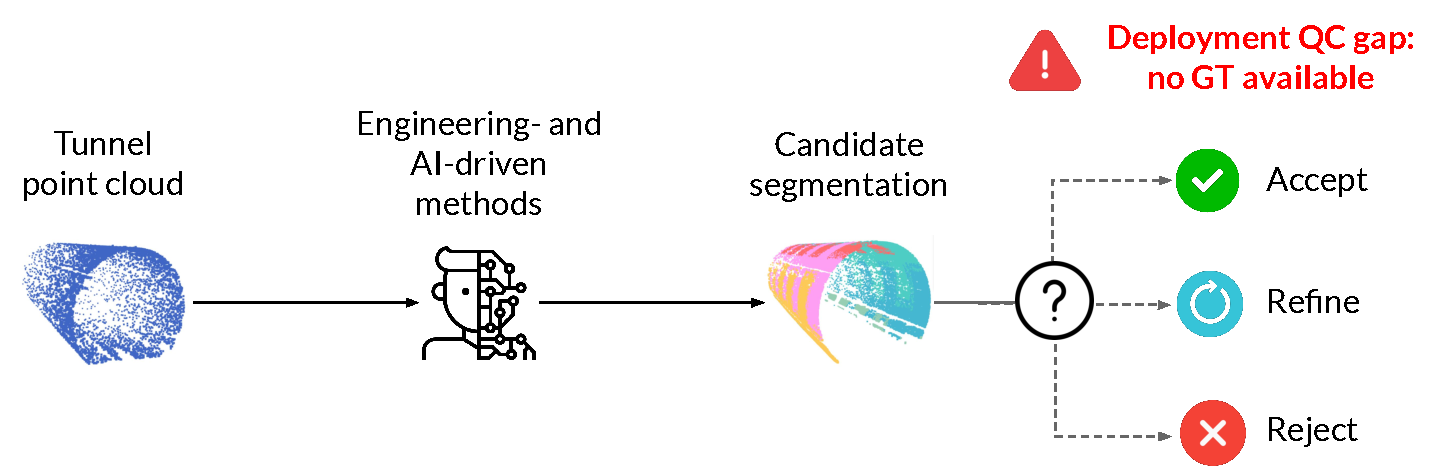
\includegraphics[width=0.8\textwidth]{figs/motivation.pdf}
\caption{Deployment QC problem: segmentation methods produce candidate outputs, but practitioners still need to decide whether to accept, refine, or flag each result without new GT labels.}
\label{fig:deployment_qc_gap}
\end{figure*}

Several point-cloud-based methods exist for tunnel-lining segmentation, but \hl{their outputs remain difficult to assess and improve when tunnel geometry or scan quality changes and ground-truth (GT) labels are unavailable}. Engineer-designed geometric pipelines rely on hand-crafted rules and thresholds with interpretable checks, yet \hl{such changes can still require manual review and parameter re-tuning}~\cite{huang2021bim,weidner2024generalized,wang2025automated}. Supervised models~\cite{su2024review,cha2024deep}, including foundation-model pipelines~\cite{bommasani2021foundation,kirillov2023sam,ye2024sam}, can output confidence or uncertainty scores learned during training, but these scores must be calibrated against task-relevant accuracy criteria before they can support deployment-time quality-control (QC) decisions: \textit{accept the output, refine it, or flag it for human review}. \hl{Without this calibration, changes in these scores may not reflect changes in segmentation accuracy, leaving failures undetected and allowing them to affect downstream assessments} (Fig.~\ref{fig:deployment_qc_gap}).

Broader studies show that segmentation accuracy can be estimated without case-specific GT labels. In medical imaging, for example, quality estimators learn from labelled development data or assess new outputs using labelled reference collections~\cite{valindria2017rca,robinson2018segmentationQuality,fournel2021segmentationQC}. However, it remains unclear how well these approaches transfer to tunnel point-cloud pipelines, where annotations are limited and parameter settings often rely on domain experts. This motivates our central research question: \emph{Can intermediate metrics from a tunnel-segmentation pipeline support accuracy estimation and parameter self-refinement without new GT labels?}

We therefore propose Proxy4Tun, a framework that uses intermediate pipeline metrics as a proxy for segmentation accuracy, enabling deployment-time QC decisions and parameter self-refinement. The proxy is constructed through a controlled calibration study using an adapted SAM4Tun pipeline~\cite{ye2025sam4tun} on three Seg2Tunnel lining families (staggered, continuous, and complex). \hl{For each family, calibration uses one labelled subset and one expert-reference parameter setting, which anchors a bounded parameter search space.}

\hl{Within these search spaces, 120 calibration runs are generated using bounded random sampling and uncertainty-guided Bayesian exploration.} This design spans both high- and low-quality outputs and helps reveal metrics that remain informative \hl{across different quality levels}. \hl{Each run records intermediate pipeline metrics alongside GT mIoU, allowing their relationships to be examined.}

\hl{These metrics fall into two groups:} preprocessing quality (PQ) and structural coherency (SC). \hl{PQ characterises the completeness and alignment of the depth representation used for segmentation}, while SC measures whether the predicted segmentation is structurally plausible. \hl{We replace the expected-ring-count residual with the number of fallback joint lines marked as assumed by the detector, then compare revised PQ/SC feature sets and unified-versus-family-isolated fits on the same 120 records.}

The selected proxy is evaluated on 54 held-out runs from 27 subsets (reference/degraded pairs) to test whether it consistently ranks the reference output above its degraded counterpart. \hl{We then rescore the already completed three-attempt candidate sets from GPT-5.6, Fable-5.1, Gemini-3.8, and adaptive-random search, applying the same} $0.01$ \hl{selection margin offline. GT mIoU is used only for retrospective evaluation. A compact control on one unseen STSD tunnel tests whether proxy-guided retention remains meaningful beyond Seg2Tunnel.}

We position Proxy4Tun as an exploratory framework for QC and self-refinement without deployment labels. \hl{Its value lies in using measurable pipeline outputs to support QC decisions and parameter refinement, with the proxy serving as an empirical signal rather than a guarantee of segmentation accuracy. The new-dataset experiment extends this evaluation beyond Seg2Tunnel, providing initial evidence of transfer that requires further testing across tunnels and lining conditions.}

The contributions of this paper are as follows:
\begin{enumerate}
\item \hl{A shared assumed-line PQ/SC accuracy proxy calibrated using one labelled subset and one expert reference per lining family for QC without deployment labels.}

\item Correct reference--degradation ranking across all 27 held-out pairs, with initial evidence of proxy transfer to an unseen tunnel with complex ring layouts.

\item \hl{Offline assumed-proxy selection of completed LLM refinements that improves held-out mean mIoU over expert-reference settings, with gains concentrated below initial GT mIoU} $\hl{0.7}$\hl{.}

\item A controlled comparison showing that LLM proposals better preserve accuracy and achieve higher retained mean mIoU than adaptive-random proposals under identical conditions.
\end{enumerate}

The rest of this paper is organised as follows. Section~\ref{sec:related} reviews related work. Section~\ref{sec:methods} presents the methodology and experimental design. Section~\ref{sec:results} reports the results, Section~\ref{sec:discussion} discusses findings and limitations, and Section~\ref{sec:conclusions} concludes.




\section{Related work}
\label{sec:related}

The review follows four connected questions: how segmentation methods adapt to changing conditions, how their outputs can be assessed without new GT labels, how calibration data can be obtained with limited annotations, and how assessment feedback can guide self-refinement.

\subsection{Tunnel segmentation and adaptation}

Methods for tunnel point-cloud segmentation range from geometric pipelines to supervised and foundation-model-based approaches. Engineer-designed pipelines use geometric rules and thresholds to identify lining surfaces and segment boundaries, but their settings may need adjustment when tunnel geometry, joint layout, or scan quality changes~\cite{huang2021bim,weidner2024generalized,wang2025automated}. PointNet++, RandLA-Net, Mask3D, and TD3D are general point-cloud neural networks that learn geometric representations from labelled 3D datasets~\cite{qi2017pointnet,hu2020randla,schult2023mask3d,kolodiazhnyi2024td3d}. Tunnel-specific supervised methods adapt these ideas with engineering constraints; LiningNet, for example, integrates structural geometry for lining segmentation~\cite{lin2025liningnet}. However, labelled tunnel data remain limited, and adapting supervised models to substantially different conditions may require additional annotations and retraining~\cite{su2024review, cha2024deep}.

Foundation-model pipelines reduce the need for task-specific training by using models pre-trained on large datasets. One practical approach is to project point clouds into two-dimensional images that can be processed by vision models. Prompt-based segmentation models include SAM~\cite{kirillov2023sam}, SAM2~\cite{ravi2024sam2}, and SEEM~\cite{zou2023segment}; infrastructure applications of such models include crack segmentation~\cite{ge2024cracksam,ye2024sam} and Scan-to-BIM workflows~\cite{wang2024omni,pan2024zero,ye2026maintenance}. For tunnel linings, SAM4Tun unfolds point clouds into panoramic images and generates template-based prompts for SAM to segment lining components without task-specific model training~\cite{ye2025sam4tun}. However, its preprocessing and prompting stages involve many interdependent parameters that encode assumptions about lining geometry and scanning conditions. When those conditions change, tuning these interdependent parameters can require substantial effort and domain expertise.

R4Tun addresses this parameter-adaptation problem by using a reference configuration, intermediate pipeline metrics, and engineering knowledge to guide LLM-proposed adjustments to SAM4Tun within prescribed parameter ranges~\cite{taoR4Tun}. Its adaptation proceeds without GT access, while the resulting segmentation accuracy is evaluated against GT offline. This supports the use of structured context to propose adjustments, but leaves a separate assessment task: determining the accuracy of the initial and adjusted outputs when new GT labels are unavailable.

\subsection{Quality estimation without new GT labels}

Existing studies estimate segmentation quality from observable properties of the data and segmentation outputs. In medical imaging, Kohlberger et al. use segmentation features to predict overlap error and Dice scores~\cite{kohlberger2012evaluating}, while Robinson et al. learn to predict quality from image--segmentation pairs~\cite{robinson2018segmentationQuality}. For point clouds, LidarMetaSeg combines input features with network confidence measures to estimate the quality of connected semantic segments in self-driving scenes~\cite{colling2021lidarmetaseg}. Consistency between processing outputs can also provide evidence, although agreement does not guarantee correctness: different LiDAR processing streams can agree on an incorrect label~\cite{bogdoll2025labelfree}. These studies suggest that data properties and output consistency can help assess quality, provided their relationship with actual accuracy is established.

Reference-based approaches provide another source of assessment evidence. Reverse Classification Accuracy (RCA) treats a new segmentation as provisional labels, trains a reverse classifier, and evaluates that classifier on labelled reference images~\cite{valindria2017rca}. Its performance on those references is used to estimate the quality of the original segmentation. ConfIC-RCA further uses retrieval of relevant reference images and in-context reverse segmentation to estimate quality~\cite{cosarinsky2026conficrca}.

These studies motivate estimating accuracy from observable processing and segmentation features, avoiding the need for new GT labels at deployment. Proxy4Tun generates calibration examples by varying pipeline parameters on a small labelled development set, using one expert reference configuration per lining family, then freezes the estimator and scores candidate outputs on new scans using only observable pipeline metrics. The remaining question is whether limited labelled tunnel data can support an estimator that remains useful on held-out data and during parameter refinement within the studied lining families.

\subsection{Calibration with limited labelled data}

Training a quality estimator requires examples spanning successful and degraded segmentations, but these examples need not require additional scan annotations. Robinson et al. generate multiple segmentations by varying model settings and reuse existing annotations to obtain quality targets~\cite{robinson2018segmentationQuality}. The same labelled input can therefore provide several examples of how processing choices affect accuracy. The challenge is to select useful settings without evaluating every possible combination.

Bayesian optimisation methods motivate incorporating prior knowledge when selecting which settings to evaluate. BOPrO encodes user beliefs about promising parameter regions, while $\pi$BO specifies a probability distribution over where the optimum is expected to lie~\cite{souza2020prior,hvarfner2022pibo}. Whereas these methods seek high-performing settings, Proxy4Tun uses uncertainty-guided Bayesian exploration to collect calibration examples across the prescribed parameter space. It starts with a space-filling design across the prescribed ranges~\cite{joe2008constructing}, fits a Gaussian-process surrogate to the observed accuracy response, and selects additional evaluations where predictive uncertainty is highest to broaden evidence across the parameter space~\cite{gramacy2009adaptive,gramacy2020surrogates}. The same development annotations are reused to calculate GT mIoU for each run.

\subsection{Feedback-guided self-refinement}

LLM-based agents can revise results by proposing changes, evaluating their effects, and using feedback to guide subsequent attempts. Self-Refine asks the model to critique and revise its output, while Reflexion records lessons from task feedback for later attempts~\cite{madaan2023selfrefine,shinn2023reflexion}. AlphaEvolve and the Darwin G\"odel Machine extend feedback-guided search to modifying programs or agent code using automated evaluation~\cite{novikov2025alphaevolve,zhang2025darwin}. However, repeated revision does not guarantee improvement. Self-correction without external feedback can fail, and increasing an imperfect proxy score can reduce performance when assessed separately~\cite{huang2024selfcorrect,gao2023overoptimization}.

Feedback can also provide diagnostic information to guide subsequent proposals. ReAct demonstrates how observations from the environment can inform subsequent actions~\cite{yao2023react}. In Proxy4Tun, PQ and SC metrics provide this feedback context for LLM reasoning: an incomplete depth map or disagreement between detected joints and predicted boundaries can suggest which stages warrant inspection.

We use a linear proxy to expose how each feature contributes to the predicted score, supporting interpretation of the proxy score~\cite{rudin2019stop}. Proxy4Tun examines whether a frozen accuracy proxy can support bounded parameter self-refinement and compares LLM and adaptive-random proposals under the same attempt budget and selection rule.

% ══════════════════════════════════════════════════════════════════════════
\section{Methodology}
\label{sec:methods}

Proxy4Tun has two phases: (i) development-time calibration on labelled scans to learn a proxy from PQ/SC metrics, and (ii) deployment-time scoring and bounded self-refinement on new scans without GT labels. Four requirements shape the design:
\begin{enumerate}
\renewcommand{\labelenumi}{\roman{enumi}.}
\item \textbf{Label efficiency.} Calibration should require minimal labelled data and expert input.
\item \textbf{Generalisation.} The proxy should remain informative across lining families and transfer to unseen datasets.
\item \textbf{Auditability.} Each feature's contribution to the proxy score should be interpretable to the LLM proposer.
\item \textbf{LLM value.} LLM proposals should improve refinement beyond random search under comparable conditions.
\end{enumerate}

\begin{figure*}[t]
\centering
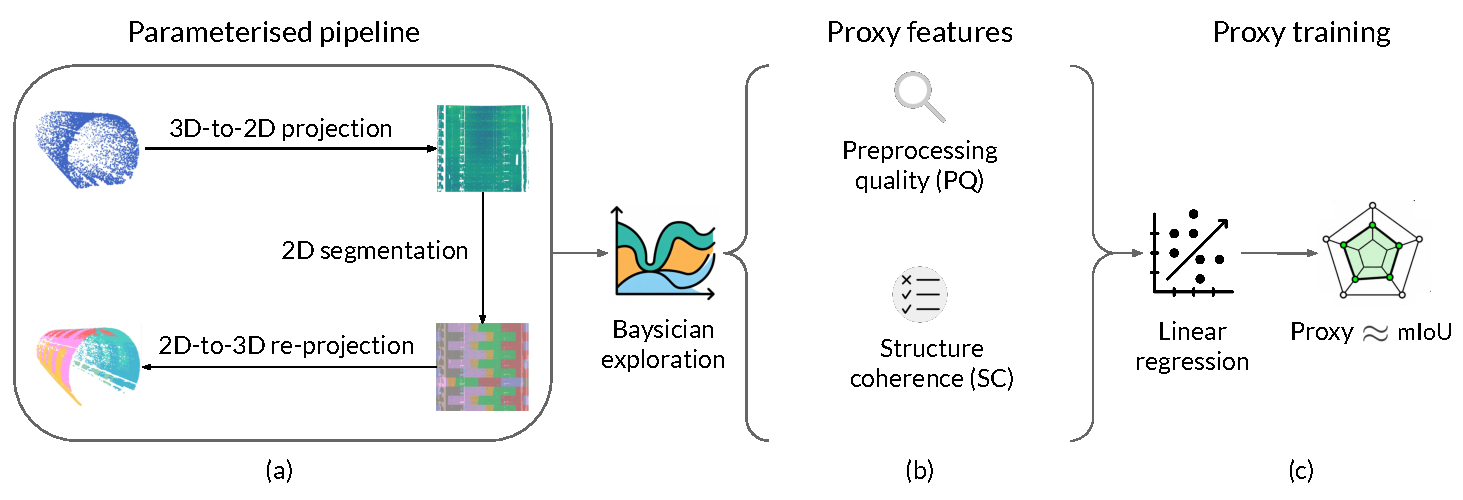
\includegraphics[width=\textwidth]{figs/intrinsics.pdf}
\caption{Development and use of the accuracy proxy. Parameter variations generate segmentation outputs with different accuracies. PQ and SC metrics from each run are paired with GT mIoU to train the proxy. Once fitted, the proxy estimates accuracy on new runs using metrics available without GT. The score is an estimate of segmentation accuracy, not a guarantee of correctness.}
\label{fig:intrinsic_proxy_scoring}
\end{figure*}


\subsection{Task definition}
\label{sec:problem-def}

Given a raw point cloud of a tunnel section, the task is to assign each point either the background label or the label of one lining block. Three block \emph{types} occur in a ring: key (K), adjacent (B), and standard (A). The label set distinguishes the individual blocks within a ring: K, B1, B2, and A1--A3 for staggered and continuous rings (six blocks), and K, B1, B2, and A1--A4 for complex rings (seven blocks), plus background in every family. Seg2Tunnel, the benchmark dataset we use, groups linings into three families (staggered, continuous, and complex). These families differ in ring geometry and acquisition conditions and, most critically for our task, in the key-block (K) layout: ring-to-ring repeating, fixed ring-wise order, and no repeating pattern (Fig.~\ref{fig:task}). 

Given an input point cloud, Proxy4Tun estimates segmentation quality using a learned proxy score computed from PQ/SC metrics. During self-refinement, it evaluates candidate configurations within a predefined parameter space and attempt budget; the proxy score then decides whether to accept the current segmentation, continue refining, or flag the result.

\begin{figure*}[t]
\centering
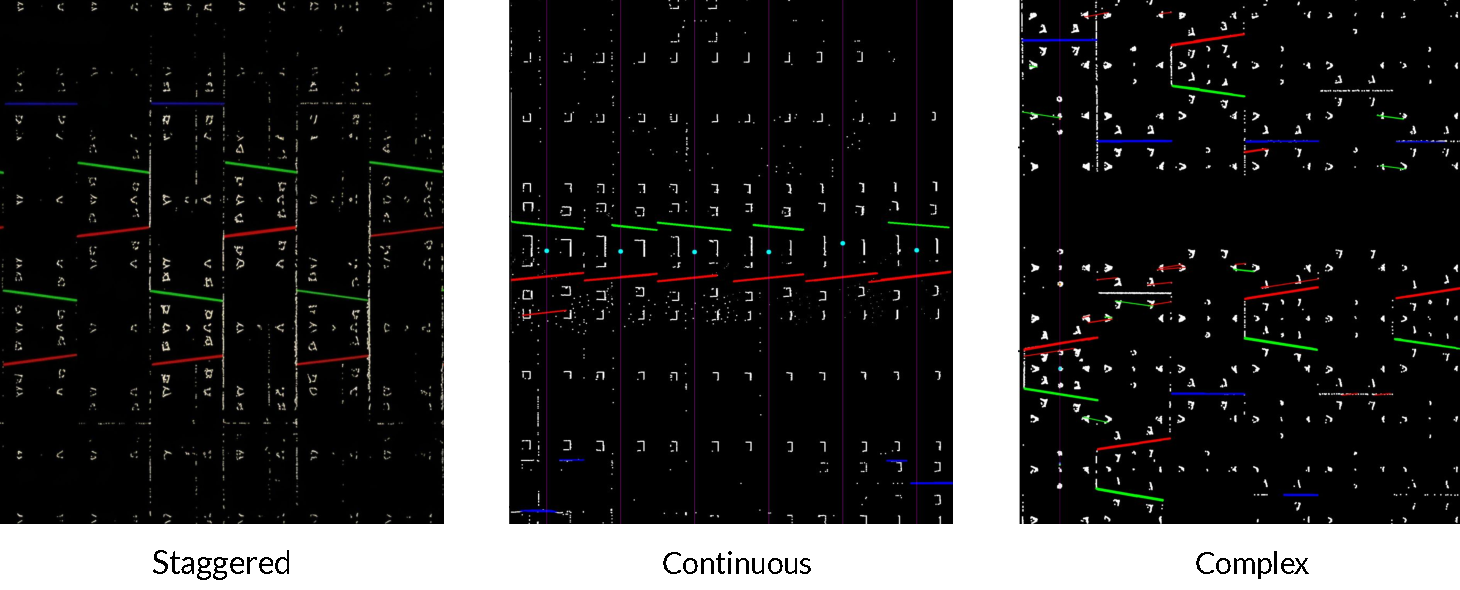
\includegraphics[width=0.8\textwidth]{figs/task.pdf}
\caption{Tunnel-lining block \emph{types} (K, B, A). Evaluation labels distinguish the individual blocks: K, B1, B2, and A1--A3 (six lining classes) or A1--A4 (seven), plus background. mIoU averages over the labels that appear, including background.} 
\label{fig:task}
\end{figure*}




\subsection{Framework overview}
\label{sec:method}

The framework links a parameterised expert-designed segmetation pipeline, a development-time procedure for learning the mIoU proxy, and a deployment-time self-refinement loop that compares candidates using the learnt proxy (Fig.~\ref{fig:intrinsic_proxy_scoring}). Throughout, the pipeline algorithms are fixed and only their parameters vary. 


\subsubsection{Segmentation pipeline}
\label{sec:pipeline}

The pipeline is adapted from SAM4Tun~\cite{ye2025sam4tun} and parameterised for the three Seg2Tunnel lining families~\cite{lin2024seg2tunnel}. Figure~\ref{fig:pipeline} illustrates the processing stages.

\begin{figure*}[t]
\centering
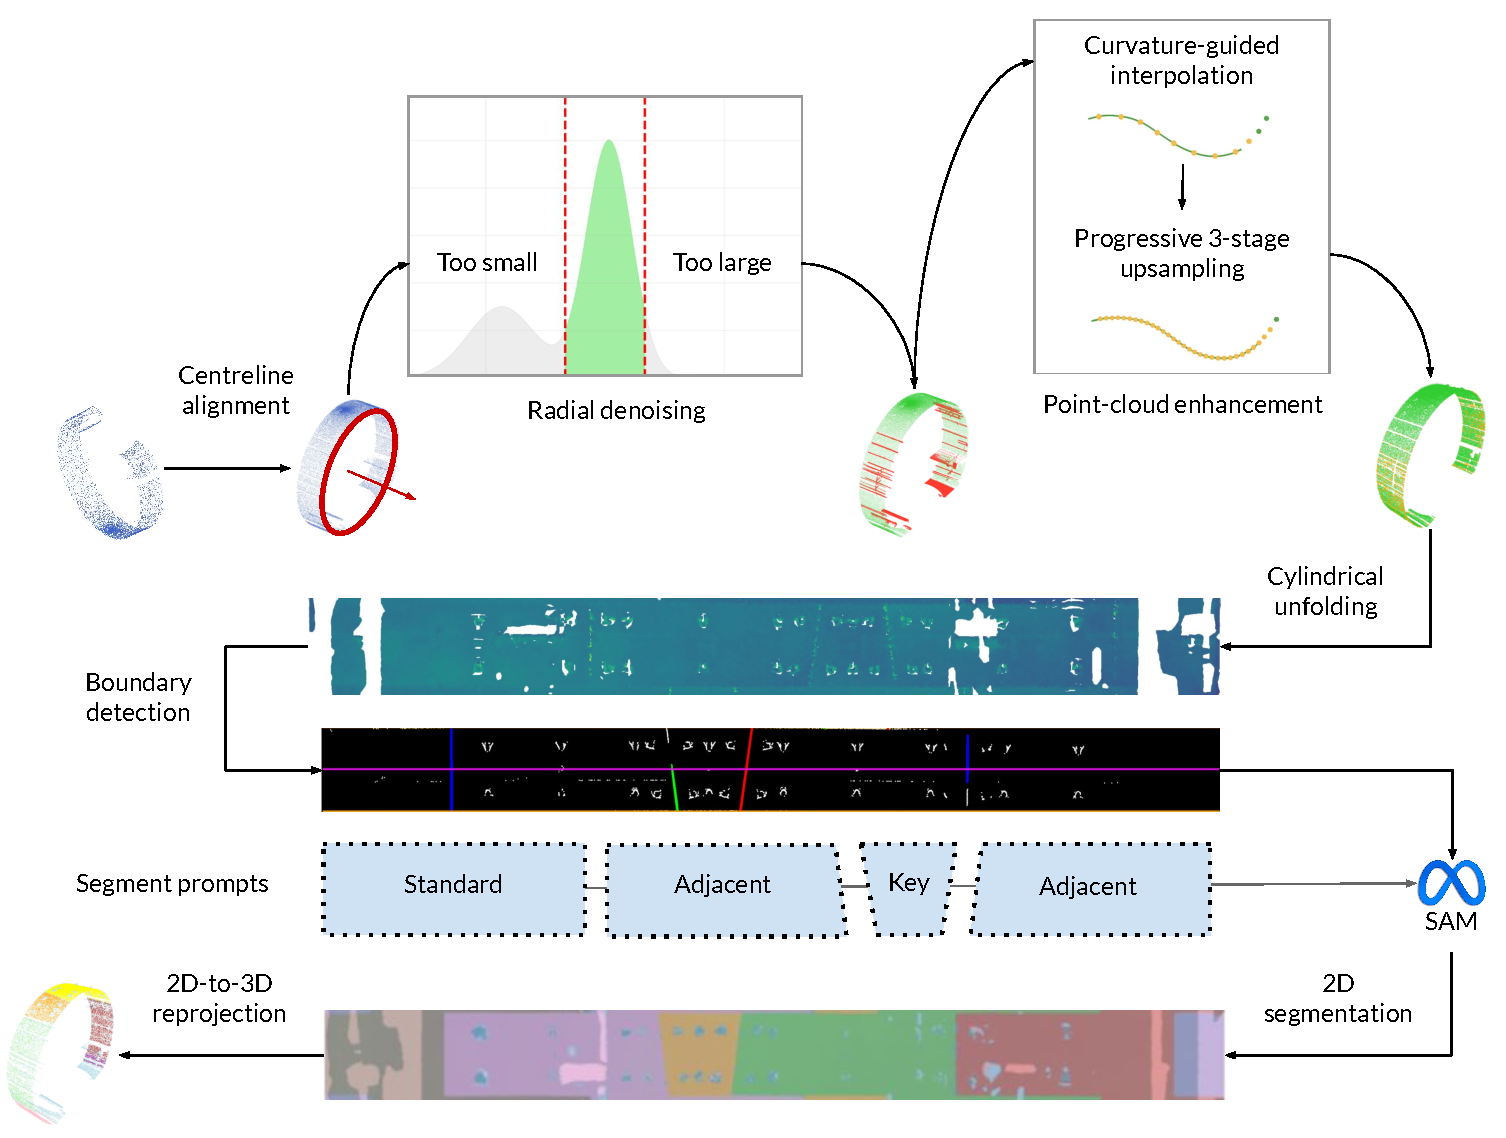
\includegraphics[width=0.98\textwidth]{figs/pipeline.pdf}
\caption{Segmentation pipeline adapted from SAM4Tun. Geometric alignment, filtering, and enhancement produce a depth representation for boundary detection and template-based SAM prompting. The resulting masks are reprojected onto the point cloud. Intermediate outputs provide PQ and SC metrics. The stage algorithms remain fixed; exploration and self-refinement adjust their parameters.}
\label{fig:pipeline}
\end{figure*}

\begin{enumerate}
\item \textbf{Unfolding.}
RANSAC-based cross-sectional ellipse fitting and centreline estimation establish a cylindrical coordinate system~\cite{fischler1981ransac}. The lining surface is represented panoramically, with depth describing radial distance from the centreline. Coordinate orientation is fixed so that block positions retain the same meaning across runs.

\item \textbf{Denoising.}
Radial masks and grid-based point-density filtering remove points inconsistent with the expected lining surface. The filtering follows the density-based principle underlying DBSCAN~\cite{ester1996dbscan}. Its settings affect both unwanted-point removal and the amount of lining data retained.

\item \textbf{Enhancement.}
Curvature-guided interpolation and progressive upsampling improve the completeness of the depth representation before detection, while preserving joint boundaries.

\item \textbf{Boundary detection.}
Orientation-specific Hough transforms identify candidate ring and block boundaries~\cite{duda1972hough}. These detections are organised according to the expected family layout.

\item \textbf{Segmentation and reprojection.}
The detected layout defines template-based prompts for SAM~\cite{kirillov2023sam}. The resulting image masks are mapped back to the point cloud to obtain three-dimensional block labels.
\end{enumerate}

This adapted pipeline is used for both calibration and self-refinement. Only its parameter settings vary within prescribed family-specific bounds; the stage algorithms and SAM model weights remain fixed (Appendix~\ref{app:anchor-parameter}). Each run produces a segmentation output and PQ/SC metrics for proxy-based quality assessment.

\subsubsection{Generating calibration examples}
\label{sec:bo-experience}
Calibration requires examples linking PQ/SC metrics to segmentation accuracy across successful and degraded parameter settings. Each lining family has an expert reference configuration, tuned by the pipeline developers on one labelled development subset before this study. We vary its parameters within prescribed bounds and reuse the same subset's annotations to calculate GT mIoU for each run, producing 120 calibration examples across three development subsets. The family references also provide the starting configurations for self-refinement.

Two sampling stages balance coverage and informativeness within each lining family. First, scrambled Sobol sampling provides 32 valid trials spread across the prescribed parameter ranges~\cite{joe2008constructing}, allowing exploration of both successful and degraded settings. Second, Bayesian exploration adds eight valid trials where a Gaussian-process (GP) model of GT mIoU has the highest predictive uncertainty~\cite{gramacy2009adaptive,gramacy2020surrogates}. We target uncertainty rather than maximise accuracy because the proxy must estimate and rank segmentation quality across a range of accuracies, rather than identify a single optimum (Appendix~\ref{app:bo-config}). Each valid run records its parameter configuration, PQ/SC metrics, and GT mIoU. Algorithm~\ref{alg:bo_exploration} and Figure~\ref{fig:b-p} summarise the procedure; Appendix~\ref{app:search-bounds} lists the parameter bounds.

\begin{figure*}[t]
\centering
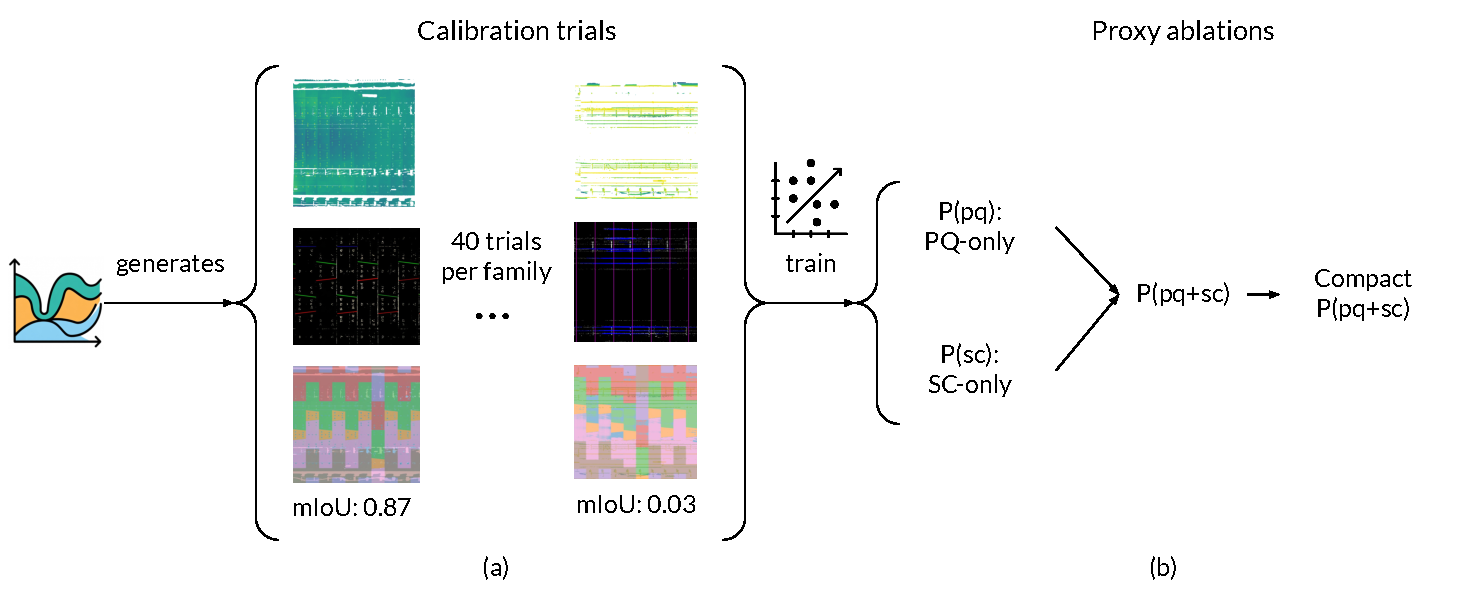
\includegraphics[width=\textwidth]{figs/b-p.pdf}
\caption{Calibration-example generation and feature comparison.
(a) Each lining family contributes 32 valid scrambled-Sobol trials
and eight valid Bayesian exploration trials selected by GP
uncertainty. All trials reuse the same development-subset annotations.
(b) The resulting metrics and GT mIoU values support comparison
of PQ-only, SC-only, combined, and compact combined feature sets
for the accuracy proxy.}
\label{fig:b-p}
\end{figure*}

\begin{algorithm}[ht]
\caption{Generating calibration examples through space-filling
sampling and Bayesian exploration}
\label{alg:bo_exploration}
\begin{algorithmic}[1]
\Require Development subset $D_f$ with GT annotations $Y_f$
\Require \hl{Reference configuration} $P_f^{\mathrm{ref}}$
\Require Parameter bounds $\Theta_f$;
         valid-trial budgets $N_0=32$, $N_1=8$;
         candidate-pool size $M=2048$
\Ensure Calibration records $\mathcal{T}_f$
\State $\mathcal{T}_f\gets\emptyset$;
       $n_0\gets0$; $n_1\gets0$
\State Initialise a scrambled-Sobol sequence
\Statex \textit{Phase 1: broad initial coverage}
\While{$n_0<N_0$}
    \State Draw the next Sobol point and map it to
           permitted parameter values $\theta\in\Theta_f$
    \State $P\gets\operatorname{Apply}
           (P_f^{\mathrm{ref}},\theta)$
    \State $R\gets\operatorname{Pipeline}(D_f,P)$
    \If{$R$ is valid and required metrics are available}
        \State $\mathbf{x}\gets\operatorname{Features}(R)$ \hl{with the revised metric definitions}
        \State $y\gets\operatorname{mIoU}(R,Y_f)$
        \State Append $(\theta,\mathbf{x},y)$
               to $\mathcal{T}_f$
        \State $n_0\gets n_0+1$
    \Else
        \State Log the failed or incomplete trial
    \EndIf
\EndWhile
\Statex \textit{Phase 2: Bayesian exploration}
\State Fit GP to the $(\theta,y)$ pairs in $\mathcal{T}_f$
\While{$n_1<N_1$}
    \State Draw $M$ random candidate settings
           $\mathcal{P}_t$ within $\Theta_f$
    \State $\theta\gets
           \arg\max_{\vartheta\in\mathcal{P}_t}
           \sigma_t(\vartheta)$
    \State $P\gets\operatorname{Apply}
           (P_f^{\mathrm{ref}},\theta)$
    \State $R\gets\operatorname{Pipeline}(D_f,P)$
    \If{$R$ is valid and required metrics are available}
        \State $\mathbf{x}\gets\operatorname{Features}(R)$ \hl{with the revised metric definitions}
        \State $y\gets\operatorname{mIoU}(R,Y_f)$
        \State Append $(\theta,\mathbf{x},y)$
               to $\mathcal{T}_f$
        \State Update GP using the expanded $\mathcal{T}_f$
        \State $n_1\gets n_1+1$
    \Else
        \State Log the failed or incomplete trial
    \EndIf
\EndWhile
\State \Return $\mathcal{T}_f$
\end{algorithmic}
\end{algorithm}

\subsubsection{PQ and SC metrics}
\label{sec:features}

Metrics form two groups that capture two aspects of pipeline quality: upstream, where the depth representation may be incomplete or misaligned (PQ), and downstream, where the recovered layout may be incoherent even when the input is sound (SC). Table~\ref{tab:candidate-features} lists the ten candidate metrics (four PQ, six SC), whose relationship with segmentation accuracy is assessed during calibration using GT mIoU. SC is particularly relevant to the complex family, where the key block does not repeat from ring to ring while the retained SC features still apply: they count the rings, match block boundaries to detected joints, and measure how much of the point cloud receives a block label. However, high structural coherence does not guarantee correctness: because joint detections also drive SAM prompting, detected joints and predicted boundaries may agree while sharing the same underlying error. Their agreement is evidence, not proof, of correctness.

\begin{table*}[t]
\caption{Candidate metrics for the mIoU accuracy proxy (four PQ, six SC). Pixel quantities refer to the 5\,mm depth-image grid. The four retained by the frozen proxy are marked $\star$. Stages: 1---unfolding; 2---denoising; 3---enhancement; 4---joint detection; 5---SAM segmentation. Combined indices indicate metrics using outputs from both stages.}
\label{tab:candidate-features}
\centering
\small
\setlength{\tabcolsep}{3pt}
\begin{tabular}{p{0.05\textwidth} p{0.27\textwidth} p{0.45\textwidth} p{0.16\textwidth}}
\toprule
Group & Measurement & Meaning & Stage \\
\midrule
PQ & Unfolding fit residual & Centreline fit error & 1 \\
 & Orientation agreement & Agreement between the inferred axis and the recorded travel direction & 1 \\
 & Point retention & Fraction of input points kept after denoising & 2 \\
 & Missing-depth rate $\star$ & Fraction of all depth-image pixels without depth after enhancement & 3 \\
\rowcolor{yellow!25}SC & Assumed-line count $\star$ & Number of fallback joint lines marked \texttt{assume} by the detector & 4 \\
 & Edge support & Fraction of label-boundary pixels within 25\,px of a depth edge & 3+5 \\
 & Correspondence score $\star$ & F1 at 15\,px between rasterised joint lines and block--block boundaries (empty detection $\Rightarrow 0$) & 4+5 \\
 & Line--boundary distance & Symmetric mean distance (capped at 200\,px) between joints and boundaries & 4+5 \\
 & Fill rate $\star$ & Fraction of all input points assigned a non-background label & 5 \\
 & Phase incoherence & Inconsistency of label ordering across rings & 5 \\
\bottomrule
\end{tabular}
\end{table*}

\subsubsection{Learning the accuracy proxy}
\label{sec:ridge-proxy}

\hl{The proxy maps PQ and SC metrics to an estimated mIoU. Following the post-hoc replacement of ring-count residual with assumed-line count, we refit ridge-regression proxies using four fixed candidate feature sets and compare them through LOFO validation.} Regularisation stabilises estimation under correlated predictors~\cite{hoerl1970ridge,pedregosa2011sklearn}, while the linear form \hl{allows the estimator to be inspected by the LLMs}. The coefficients represent fitted associations, not causal prescriptions for parameter changes. We choose this model form for interpretable feedback and do not claim predictive superiority over nonlinear alternatives.

For a feature vector $\mathbf{x}\in\mathbb{R}^{d}$, the prediction is
\begin{equation}
\hat{y}(\mathbf{x})
=
b+\sum_{j=1}^{d}
w_j\frac{x_j-\mu_j}{s_j},
\label{eq:ridge-proxy}
\end{equation}
where $d$ is the number of features, $\mu_j$ and $s_j$ are the training-set mean and standard deviation of feature $j$, $w_j$ is its fitted coefficient, and $b$ is the intercept. Coefficients are fitted by minimising squared prediction error with an $\ell_2$ penalty of strength $\alpha$.

\hl{We compare four fixed feature sets: PQ-only} $P(q)$\hl{, revised SC-only} $P(c)$\hl{, revised combined} $P(q{+}c)$\hl{, and the compact combined model (Table}~\ref{tab:proxy-ablation}\hl{). The substitution was post hoc; the compact set was not prespecified as the winner of this revised comparison.} Each LOFO fold trains on two families and evaluates on the third, with feature scaling, penalty selection, and coefficient fitting restricted to the training families. Predictions across the three held-out folds are pooled to calculate Spearman $\rho$ and MAE over all 120 calibration runs; per-family $\rho$ is also reported. The feature set with the highest pooled LOFO $\rho$ is selected, and the final model is fitted on all 120 calibration runs and frozen. Algorithm~\ref{alg:proxy} summarises model development and deployment scoring.

\begin{table}[ht]
\caption{\hl{Revised proxy feature sets compared under LOFO validation.}}
\label{tab:proxy-ablation}
\centering
\begin{tabular}{p{0.38\columnwidth} p{0.52\columnwidth}}
\toprule
Model & Definition \\
\midrule
$P(q)$ & Four PQ features \\
$P(c)$ & Six SC features \\
$P(q{+}c)$ & All ten candidate features \\
\rowcolor{yellow!25}Compact $P(q{+}c)$ & Four fixed features: one PQ and three SC \\
\bottomrule
\end{tabular}
\end{table}

\begin{algorithm}[ht]
\caption{Proxy calibration and deployment scoring}
\label{alg:proxy}
\begin{algorithmic}[1]
\Require Calibration records $\mathcal{T}=\bigcup_f\mathcal{T}_f$; \hl{fixed revised candidate feature sets}; fixed feature-extraction conventions
\Ensure Frozen proxy $g$ and deployment score $\hat{y}$
\For{each candidate feature set $V$}
    \For{each held-out family $f$}
        \State Use the other two families as training data
        \State Fit feature scaling and select $\alpha$ using only the training data
        \State Fit ridge regression and predict the held-out family's mIoU
        \State Clip predictions to $[0,1]$
    \EndFor
    \State Pool predictions across the three folds
    \State Record pooled Spearman $\rho$ and MAE, and per-family $\rho$
\EndFor
\State Select the feature set with the highest pooled LOFO $\rho$
\State Fit final scaling and ridge regression on all 120 calibration records
\State Freeze feature definitions, order, scaler, coefficients, and intercept as $g$
\Statex
\State \hl{Receive a completed run} $r$
\State $\mathbf{x}\gets\operatorname{Features}(r)$ \hl{in the frozen feature order}
\State $\hat{y}\gets\min(1,\max(0,g(\mathbf{x})))$
\State \Return $\hat{y}$
\end{algorithmic}
\end{algorithm}


\subsection{\hl{Assumed-proxy rescoring of parameter self-refinement}}
\label{sec:agent-design}

\hl{The proxy estimates accuracy but does not decide which parameters to change. In the completed campaigns, each LLM agent proposed bounded parameter changes from the family reference, intermediate outputs, PQ/SC metrics, proxy feedback, and engineering notes (Appendices}~\ref{app:ontology} \hl{and}~\ref{app:prompt}\hl{).}

\paragraph{Shared protocol.}
\hl{The completed campaign contains one expert-reference start and three proposal attempts per arm for each of 27 subsets, without admission screening or early stopping. The revision holds all proposals and pipeline outputs fixed and changes only offline scoring and selection.}

\paragraph{Adaptive-random control.}
The control samples the number of parameters to change from an empirical distribution obtained from an earlier LLM pilot, then randomly selects parameters and values within the allowed bounds (Appendix~\ref{app:random-search}). This distribution is frozen before the experiment. Random updates are applied to the retained configuration without using intermediate metrics or images to guide sampling. In all arms, however, unfolding parameters are eligible for modification only when the starting centreline residual exceeds $10\,\mathrm{cm}$. The comparison evaluates proposal strategies under common constraints; it does not isolate LLM reasoning from differences in proposal size or parameter choice.

\paragraph{Execution and feedback.}
\hl{The historical campaigns checked and executed each proposal, recording outputs and metrics. The LLM records informed their subsequent historical attempts. The assumed-line proxy does not regenerate that feedback; it rescores the completed candidate set.}

\paragraph{Retention.}
\hl{For the assumed-line analysis, all saved starts and candidates are rescored offline. The highest proxy score is selected; if candidates lie within the predefined margin of} $\hl{0.01}$ \hl{of that maximum, the earliest round is retained. The same rule applies to all arms and no proposal is rerun.}

\begin{figure*}[t]
\centering
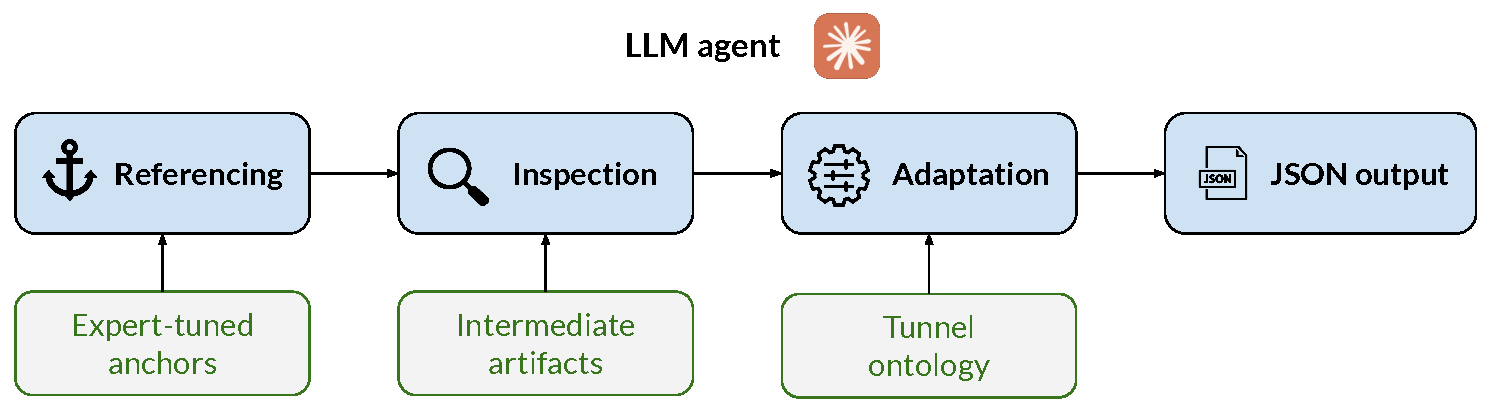
\includegraphics[width=0.8\textwidth]{figs/agent.pdf}
\caption{\hl{Historical LLM candidate generation. The assumed-line analysis does not regenerate proposals; it rescores the saved outputs from these completed campaigns.}}
\label{fig:agent}
\end{figure*}

\begin{algorithm}[ht]
\caption{\hl{Offline assumed-proxy rescoring and selection}}
\label{alg:reflective_adaptation}
\begin{algorithmic}[1]
\Require \hl{Saved expert-reference start and three saved candidates; frozen assumed-line proxy}
\Ensure Retained configuration, segmentation output, and proxy score
\State \hl{Load the saved expert-reference start and its three saved candidates}
\State \hl{Rescore all four outputs with the frozen assumed-line proxy}
\For{attempt $=1,2,3$}
    \State \hl{Read the saved candidate's metrics and assumed-line count}
    \State \hl{Compute its clipped assumed-line proxy score}
\EndFor
\State \hl{Let} $s_{\max}$ \hl{be the maximum score among the start and candidates}
\State \hl{Return the earliest output with score} $\geq s_{\max}-0.01$
\end{algorithmic}
\end{algorithm}


\subsection{Experimental setup}
\label{sec:exp-setup}

\subsubsection{Dataset and reference configurations}
\label{sec:dataset}
We use 30 ten-ring subsets from five parent tunnels in Seg2Tunnel, covering staggered, continuous, and complex lining families~\cite{lin2024seg2tunnel}. One labelled development subset per family supplies 40 calibration runs; the remaining 27 subsets are held out for evaluation (Table~\ref{tab:dataset}). A single proxy is fitted to calibration runs pooled across all three lining families and evaluated on the 27 held-out subsets. Where we report bootstrap confidence intervals, we account for shared geometry and acquisition conditions by resampling at the parent-tunnel level unless stated otherwise (Section~\ref{sec:sensitivity}).


Each expert family reference was tuned by the pipeline developers on the corresponding development subset, with its annotations available, and established before this study. It provides the basis for calibration and the unchanged starting configuration for held-out evaluation and self-refinement. Development annotations support reference assessment and supply calibration targets; held-out annotations are used only for retrospective evaluation. Appendices~\ref{app:anchor-parameter} and~\ref{app:search-bounds} list the reference configurations and exploration bounds, respectively.

\begin{table*}[t]
\caption{Development and held-out subsets. One labelled development subset per family supplies the calibration trials; nine other subsets per family form the held-out evaluation data.}
\label{tab:dataset}
\centering
\begin{tabular}{p{0.22\textwidth} p{0.24\textwidth} p{0.22\textwidth} p{0.22\textwidth}}
\toprule
Property & Staggered (T1, T2) & Continuous (T3) & Complex (T4, T5) \\
\midrule
Inner diameter & 5.5\,m & 5.9\,m & 7.5\,m \\
Ring length & 1.2\,m & 1.2\,m & 1.8\,m \\
Blocks per ring & 6 & 6 & 7 \\
Key-block layout & Ring-to-ring repeating pattern & Fixed ring-wise order & No repeating pattern \\
Scanning & Single-station & Multi-station & Single-station, offset \\
Development subset & 2-1 & 3-1 & 5-1 \\
Calibration runs & 40 & 40 & 40 \\
Held-out subsets & 1-1 to 1-5; 2-2 to 2-5 & 3-2 to 3-10 & 4-1-to 4-5; 5-2 to 5-5 \\
\bottomrule
\end{tabular}
\end{table*}


\subsubsection{Feature and model comparisons}
\label{sec:comparators}

\hl{We use the 120 calibration runs for four checks. First, we compare the revised feature sets by LOFO (Table}~\ref{tab:proxy-ablation}\hl{). Second, we shuffle GT mIoU within each family and repeat LOFO fitting 20 times. Third, a learning curve subsamples 5--40 runs per family over 20 deterministic repeats. Fourth, matched repeated five-fold CV compares one unified compact model with family-isolated compact models; every model is scored on the same held-out fold, over 20 repeats.}

\subsubsection{Paired degradation test}
\label{sec:stress-test}

For each of the 27 held-out subsets, we run the family reference and a deliberately degraded configuration (Appendix~\ref{app:degradation}). Both configurations process the same input point cloud, avoiding differences between scans. GT mIoU is calculated afterwards to confirm degradation. We evaluate how accurately the frozen proxy estimates mIoU and whether it ranks each reference output above its degraded counterpart. This tests ranking under controlled degradation rather than reliability on naturally occurring failures.

\subsubsection{Self-refinement against family-specific references}
\label{sec:poc-protocol}

\hl{We compare four completed proposal arms on all 27 held-out subsets: GPT-5.6, Fable-5.1, Gemini-3.8, and adaptive-random search. Each historical arm contains the same expert-reference start and three attempts. The assumed-line substitution is evaluated by offline rescoring and reselection only; no LLM proposal or pipeline run is repeated.} Table~\ref{tab:poc-config} lists the study configuration.

\hl{The completed campaigns logged all 324 proposals and outcomes} ($27$ \hl{subsets} $\times 4$ \hl{arms} $\times 3$ \hl{attempts}), \hl{comprising 243 LLM and 81 adaptive-random proposals. The assumed-line analysis reads these records without new model calls or pipeline runs.}

\begin{table}[ht]
\caption{Self-refinement study configuration.}
\label{tab:poc-config}
\centering
\begin{tabular}{p{0.35\columnwidth} p{0.55\columnwidth}}
\toprule
Setting & Value \\
\midrule
Proposal arms & GPT-5.6; Fable-5.1; Gemini-3.8; adaptive-random search \\
LLM identifiers & \texttt{gpt-5.6-sol-medium}; \texttt{claude-fable-5-1-thinking-high}; Gemini~3.8 as the active agent model \\
Interface & One coding-agent session per subset and LLM arm, resumed across attempts \\
Starting configuration & Expert family reference \\
Evaluation cases & All 27 held-out subsets \\
Context (LLM arms) & Engineering notes, pipeline outputs, PQ/SC metrics, and proxy scores; no GT \\
Budget & Three proposal attempts per subset and arm \\
Early stopping & None \\
Output & One JSON parameter update per attempt, with a rationale for LLM arms \\
Failure handling & Invalid or failed attempts consume budget; retained output remains unchanged \\
\rowcolor{yellow!25}Retention & Highest assumed-line score; within $0.01$ of the maximum, keep the earliest round \\
\bottomrule
\end{tabular}
\end{table}


\subsubsection{Evaluation metrics}
\label{sec:metrics}

Segmentation accuracy is evaluated retrospectively against GT using point-wise semantic mIoU:
\begin{equation}
\operatorname{IoU}_c
=
\frac{\operatorname{TP}_c}
{\operatorname{TP}_c+\operatorname{FP}_c+\operatorname{FN}_c},
\qquad
\operatorname{mIoU}
=
\frac{1}{C}\sum_{c=1}^{C}\operatorname{IoU}_c,
\end{equation}
where $\operatorname{TP}_c$, $\operatorname{FP}_c$, and $\operatorname{FN}_c$ are the true-positive, false-positive, and false-negative point counts for label $c$, and $C$ is the number of labels included in the average for that subset (labels present in either GT or prediction, including background). In this study, $C=7$ for staggered and continuous subsets and $C=8$ for complex subsets.

Proxy performance is measured by Spearman $\rho$ for agreement with GT accuracy rankings and mean absolute error (MAE), defined as the mean absolute difference between predicted and GT mIoU. In the paired degradation test, we also report the proportion of pairs in which the reference receives a higher proxy score than its degraded counterpart; ties count as failures.

For self-refinement, we report proxy scores and GT mIoU before and after refinement. For each proposal strategy, we subtract each subset's initial GT mIoU from its final GT mIoU and average these changes across the 27 subsets. \hl{Averaging across the 27 subsets gives equal weight to each lining family, since each contributes nine subsets.} Proposal quality is assessed relative to the expert-reference start: a proposal is classified as harmful if its GT mIoU is more than $0.05$ lower than the starting value.

\hl{The 324 saved proposals also provide a non-constructed gate test. We report proxy--mIoU Spearman correlation, MAE, and recall for severe failures. Operating bands are evaluated at flag below} $\hl{0.4}$\hl{, refine from} $\hl{0.4}$ \hl{through} $\hl{0.7}$\hl{, and accept above} $\hl{0.7}$\hl{; these bands do not control admission to the completed three-attempt panel.}


\subsubsection{Statistical uncertainty}
\label{sec:sensitivity}

\hl{The reported mean gain is the unweighted mean of the 27 subset changes. For its interval, each parent tunnel is reduced to a mean gain; the five tunnel means are then resampled with replacement and averaged with equal weight. Table}~\ref{tab:arm-compare} \hl{reports the resulting percentile interval.} Intervals are interpreted cautiously because only five parent tunnels are available.

\subsubsection{Sensitivity to LLM choice}
\label{sec:llm-sensitivity}

\hl{We assess sensitivity to proposer choice by applying the same assumed-proxy offline selector to GPT-5.6, Fable-5.1, and Gemini-3.8 candidates generated under identical starts, bounds, and budgets.} We compare final mIoU, changes from the expert-reference baseline, harmful-proposal rates, and the numbers of improved, unchanged, and worsened subsets. These comparisons examine whether the observed benefits are consistent across the three models or concentrated in one. Each model is evaluated once per subset, so the analysis describes differences between models rather than variability across repeated sessions.


\section{Results}\label{sec:results}
% ══════════════════════════════════════════════════════════════════════════

The results follow the three questions of Section~\ref{sec:exp-setup}: whether PQ and SC carry accuracy information that transfers across families, whether the frozen proxy separates references from degradations on \hl{held-out tunnel sections}, and whether it can guide refinement of already-strong references. A residual error analysis then examines failure modes that the four-feature proxy does not reliably detect.

\subsection{Proxy calibration and feature ablation}
\label{sec:main-results}
\label{sec:proxy-ablation-results}

\hl{The selected proxy contains three SC metrics (correspondence F1@15, segmentation fill rate, and assumed-line count) and one PQ metric (depth-map missing-pixel fraction). With training-standardised inputs, its refitted equation is}
\begin{hlbox}
\begin{equation}
\begin{aligned}
\hat{y}={}&0.358867+0.088443z_{\mathrm{corr}}+0.105800z_{\mathrm{fill}}\\
&-0.021558z_{\mathrm{assume}}-0.033997z_{\mathrm{nan}}.
\end{aligned}
\label{eq:four-proxy}
\end{equation}
\end{hlbox}
\begin{figure*}[t]
\centering
\begin{hlbox}
\centering
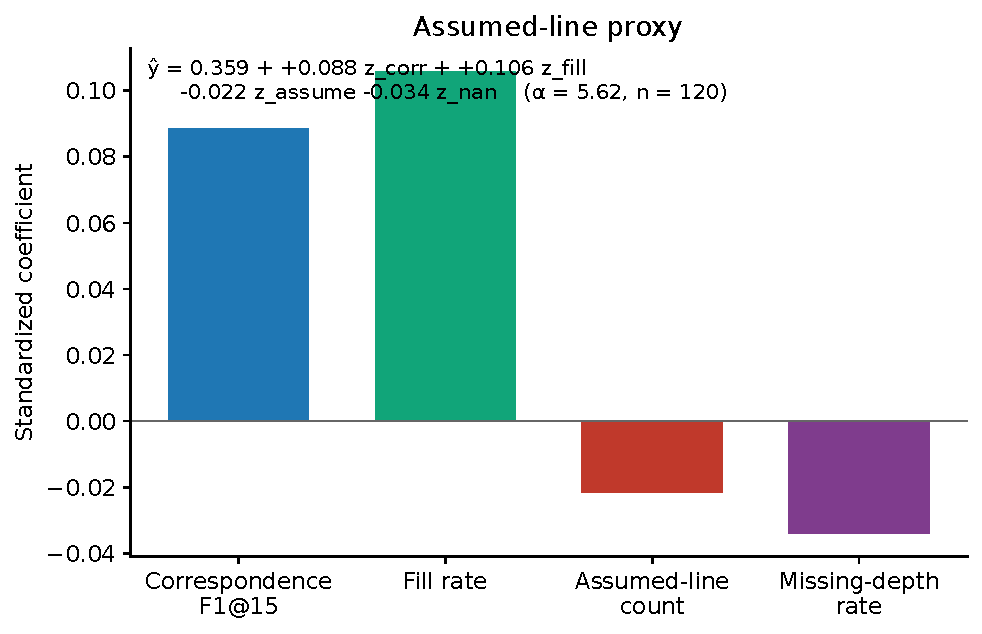
\includegraphics[width=0.98\linewidth]{figs/assume_proxy_formula.pdf}
\end{hlbox}
\caption{\hl{Standardised assumed-line proxy and fitted coefficient contributions on the 120 calibration records.}}\label{fig:assume-proxy-formula}
\end{figure*}
\hl{Each} $z$ \hl{uses the calibration-set mean and standard deviation. RidgeCV selects} $\alpha=\hl{5.623}$\hl{. Greater correspondence and coverage increase estimated mIoU, while assumed fallback lines and missing depth decrease it, holding the other metrics constant. These are conditional associations, not causal effects.}



\begin{table*}[t]
\caption{Proxy calibration and LOFO transfer (four-feature compact model). \hl{The} $\pm$ \hl{value is the standard deviation across the 20 within-family shuffles.}}\label{tab:proxy-calibration}
\begin{tabular*}{\textwidth}{@{\extracolsep{\fill}} l c c @{}}
\toprule
Setting & MAE & Spearman \\
\midrule
\rowcolor{yellow!25}Training fit ($n = 120$) & 0.108 & 0.863 \\
\rowcolor{yellow!25}Permutation control (20 shuffles, LOFO four-feature) & -- & $-0.122\pm0.093$ \\
\rowcolor{yellow!25}Leave-one-family-out (four-feature) & 0.145 & 0.754 \\
\bottomrule
\end{tabular*}
\end{table*}

\hl{Table}~\ref{tab:proxy-calibration} \hl{reports the refit. Spearman} $\rho$ \hl{decreases from} $\hl{0.863}$ \hl{in training to} $\hl{0.754}$ \hl{under LOFO. By family, LOFO correlation is} $\hl{0.883}$ \hl{(staggered),} $\hl{0.479}$ \hl{(continuous), and} $\hl{0.861}$ \hl{(complex). The within-family permutation control gives} $\rho=\hl{-0.122\pm0.093}$\hl{, so the observed association is not explained by family identity alone.}

\hl{Table}~\ref{tab:ablation-results} \hl{compares the revised sets. SC exceeds PQ} ($\rho=\hl{0.715}$ \hl{vs.} $\hl{0.615}$)\hl{, and the revised ten-feature set reaches} $\hl{0.744}$\hl{. The compact model has the highest pooled LOFO correlation} ($\hl{0.754}$) \hl{and lowest MAE} ($\hl{0.145}$) \hl{among these four post-hoc revised conditions, although it is not best on every family.}

\begin{table*}[t]
\caption{Proxy feature-set comparison under LOFO fitting. \hl{Family columns are the Spearman correlation on that held-out family.}}\label{tab:ablation-results}
\begin{tabular*}{\textwidth}{@{\extracolsep{\fill}} l c cccc c @{}}
\toprule
Condition & \#Features & Pooled $\rho$ & Staggered & Continuous & Complex & LOFO MAE \\
\midrule
$P(q)$ (PQ only) & 4 & 0.615 & 0.595 & 0.551 & 0.466 & 0.166 \\
\rowcolor{yellow!25}$P(c)$ (revised SC only) & 6 & 0.715 & 0.834 & 0.358 & 0.866 & 0.155 \\
\rowcolor{yellow!25}$P(q{+}c)$ (revised combined) & 10 & 0.744 & 0.869 & 0.263 & 0.936 & 0.148 \\
\rowcolor{yellow!25}Compact $P(q{+}c)$ (deployed) & \textbf{4} & \textbf{0.754} & \textbf{0.883} & \textbf{0.479} & \textbf{0.861} & \textbf{0.145} \\
\bottomrule
\end{tabular*}
\end{table*}

\begin{figure*}[t]
\centering
\begin{hlbox}
\centering
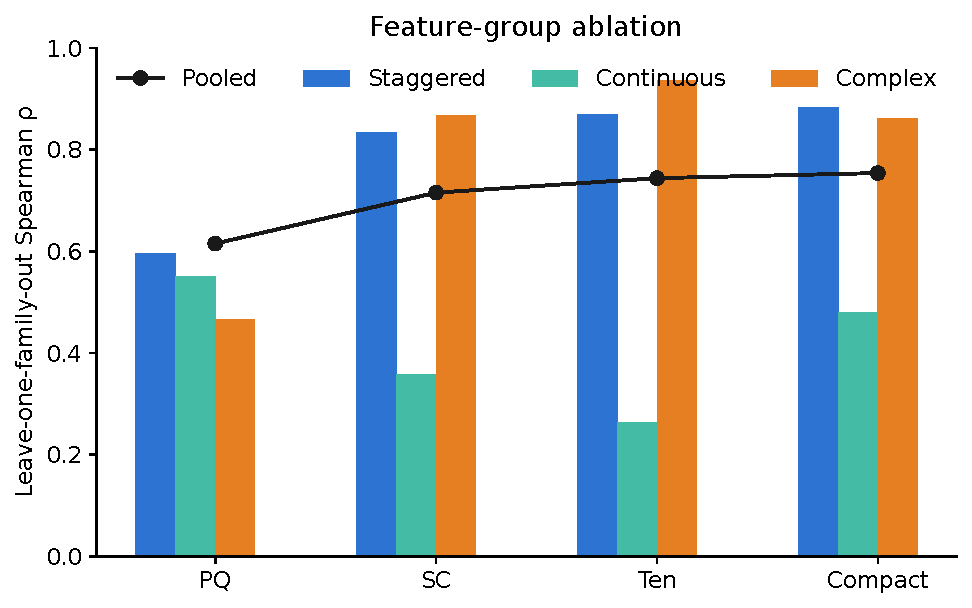
\includegraphics[width=0.98\linewidth]{figs/assume_feature_ablation.pdf}
\end{hlbox}
\caption{\hl{Revised feature-group LOFO ablation after replacing ring-count residual with assumed-line count.}}\label{fig:assume-feature-ablation}
\end{figure*}

\begin{table*}[t]
\caption{\hl{Matched repeated five-fold CV of unified and family-isolated compact proxies (20 repeats). Overall values are mean} $\pm$ \hl{SD; family rows are means.}}\label{tab:family-isolation}
\begin{tabular*}{\textwidth}{@{\extracolsep{\fill}} l cccc @{}}
\toprule
Evaluation set & Unified $\rho$ & Isolated $\rho$ & Unified MAE & Isolated MAE \\
\midrule
\rowcolor{yellow!25}Overall & $0.850\pm0.002$ & $0.885\pm0.008$ & $0.115\pm0.001$ & $0.095\pm0.003$ \\
\rowcolor{yellow!25}Staggered & 0.892 & 0.923 & 0.126 & 0.075 \\
\rowcolor{yellow!25}Continuous & 0.703 & 0.682 & 0.112 & 0.109 \\
\rowcolor{yellow!25}Complex & 0.846 & 0.822 & 0.106 & 0.100 \\
\bottomrule
\end{tabular*}
\end{table*}

\begin{figure*}[t]
\centering
\begin{hlbox}
\centering
\includegraphics[width=0.98\linewidth]{figs/assume_family_isolation.pdf}
\end{hlbox}
\caption{\hl{Matched repeated-CV comparison of the unified and family-isolated compact proxies.}}\label{fig:assume-family-isolation}
\end{figure*}

\hl{Family-isolated fits have the higher pooled correlation, driven by staggered, whereas the unified model ranks continuous and complex folds better (Table}~\ref{tab:family-isolation}\hl{). We retain the unified proxy as the shared cross-family deployment model rather than claiming it is uniformly superior. The learning curve gives mean LOFO} $\rho=\hl{0.641\pm0.174}$ \hl{with five runs per family,} $\hl{0.699\pm0.086}$ \hl{with ten, and} $\hl{0.754}$ \hl{with all 40.}

\subsection{Discriminating Reference vs. Degraded Outputs}
\label{sec:holdout}

\hl{The frozen assumed-line proxy separates reference and degraded outputs: the lowest reference score is} $\hl{0.412}$\hl{, while the highest degraded score is} $\hl{0.179}$\hl{. On all 54 runs, Spearman} $\rho=\hl{0.789}$ \hl{and MAE is} $\hl{0.106}$\hl{. A threshold of} $\hl{0.4}$\hl{, chosen retrospectively within this gap, flags all 27 degradations and no references. These constructed pairs demonstrate discrimination but do not independently validate the threshold.}

\begin{table}[ht]
\caption{Holdout fidelity of the four-feature proxy (54 runs: 27 family-specific references and 27 constructed degraded overlays).}
\label{tab:holdout-fidelity}
\footnotesize
\setlength{\tabcolsep}{2pt}
\begin{tabular*}{\tblwidth}{@{\extracolsep{\fill}} l c @{}}
\toprule
Metric & Value \\
\midrule
\textit{Ranking agreement} \\
\rowcolor{yellow!25}Spearman $\rho$ & 0.789 \\
\rowcolor{yellow!25}Bootstrap 95\% CI (subset; pairs together) & $[0.711,\,0.858]$ \\
\addlinespace
\textit{Prediction error} \\
MAE (overall) & 0.106 \\
\addlinespace
\textit{Paired ranking and retrospective flagging} \\
Pair ranking (reference $>$ degraded) & 27/27 \\
Retrospective threshold $\hat{y}<0.4$: precision / recall & 1.000 / 1.000 \\
\bottomrule
\end{tabular*}
\end{table}

\begin{figure*}[t]
\centering
\begin{hlbox}
\centering
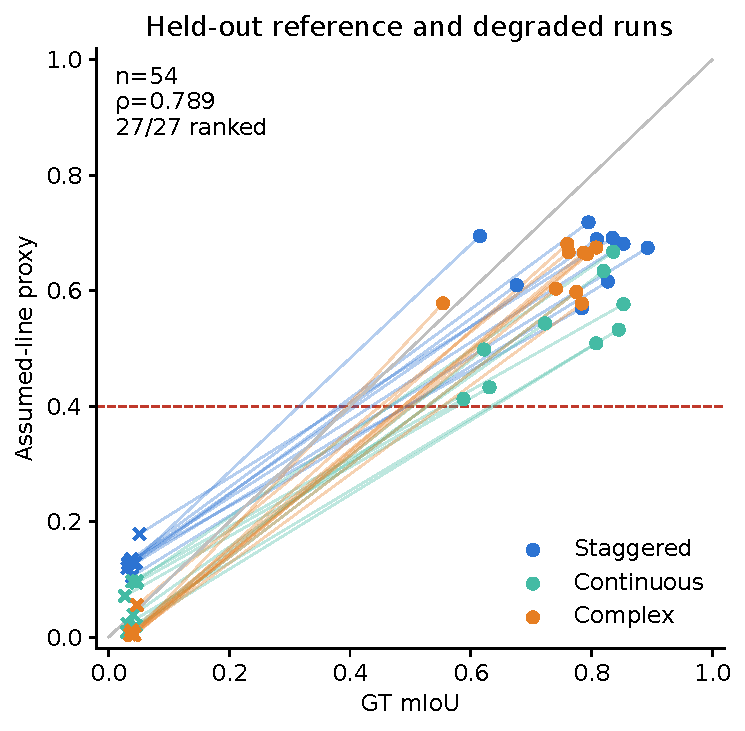
\includegraphics[width=0.98\linewidth]{figs/assume_holdout_ranking.pdf}
\end{hlbox}
\caption{\hl{Assumed-line proxy scores for the 27 held-out reference--degraded pairs.}}\label{fig:assume-holdout}
\end{figure*}

\subsection{Natural-proposal gate}
\label{sec:natural-gate}

\hl{The 324 saved, non-constructed proposals give proxy--mIoU Spearman} $\rho=\hl{0.516}$ \hl{(parent-cluster 95\% CI} $\hl{[0.400,\,0.680]}$\hl{) and MAE} $\hl{0.141}$\hl{. All 18 proposals with GT mIoU below} $\hl{0.3}$ \hl{score below the retrospective flag threshold} $\hl{0.4}$\hl{. At the 27 expert-reference starts, the flag/refine/accept bands produce} $\hl{0/26/1}$\hl{. These naturally occurring candidates supplement, but do not replace, the constructed-pair test.}

\begin{table}[ht]
\caption{\hl{Severe-failure recall among 324 saved proposals as the proxy flag threshold varies.}}\label{tab:natural-gate}
\begin{tabular*}{\tblwidth}{@{\extracolsep{\fill}} l ccc @{}}
\toprule
Flag threshold & GT $<0.3$ & GT $<0.4$ & GT $<0.5$ \\
\midrule
\rowcolor{yellow!25}0.30 & 1.000 & 0.833 & 0.677 \\
\rowcolor{yellow!25}0.40 & 1.000 & 0.958 & 0.839 \\
\rowcolor{yellow!25}0.50 & 1.000 & 1.000 & 0.871 \\
\bottomrule
\end{tabular*}
\end{table}

\begin{figure*}[t]
\centering
\begin{hlbox}
\centering
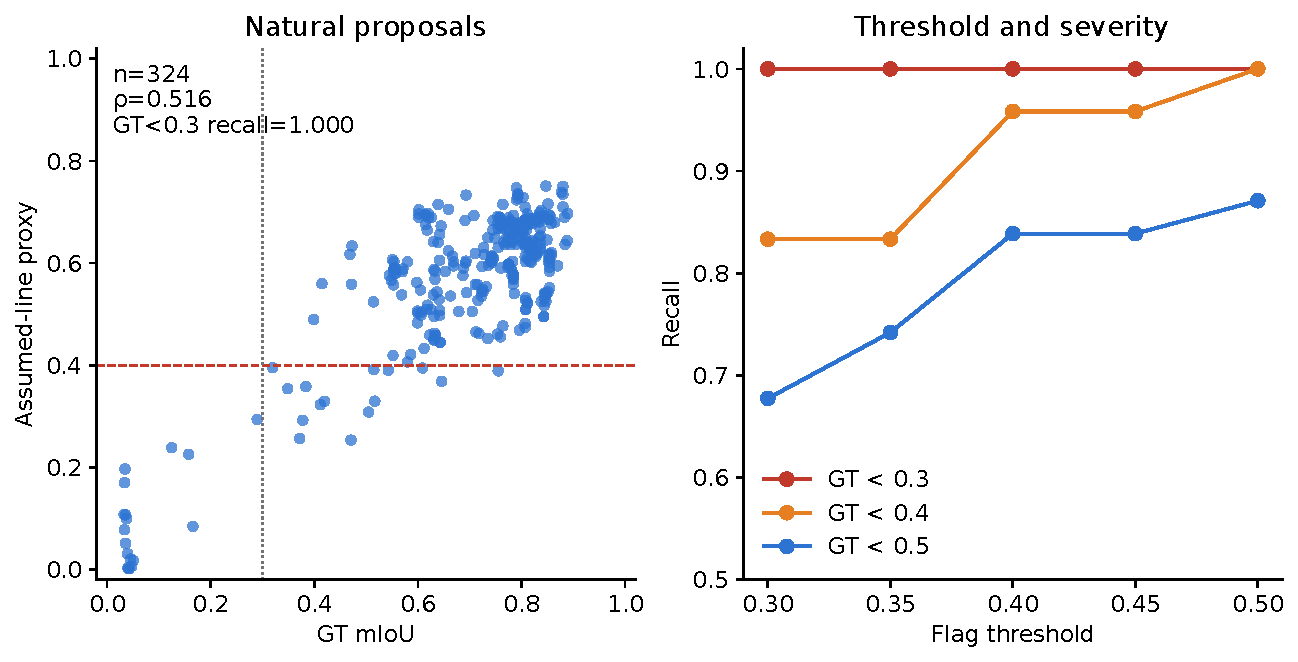
\includegraphics[width=0.98\linewidth]{figs/assume_natural_gate.pdf}
\end{hlbox}
\caption{\hl{Proxy--mIoU association and threshold--severity sensitivity on 324 saved proposals.}}\label{fig:assume-natural-gate}
\end{figure*}



\subsection{Self-refinement from expert-reference configurations}
\label{sec:poc-verification}

\begin{table*}[t]
\caption{\hl{Offline assumed-proxy reselection on all 27 held-out family-specific references. Means give equal weight to all subsets. The 95\% CI resamples five parent-tunnel mean gains. Up/same/down uses GT mIoU changes above} $0.005$\hl{, within} $\pm0.005$\hl{, and below} $-0.005$\hl{.}}\label{tab:arm-compare}
{\small
\begin{tabular*}{\textwidth}{@{\extracolsep{\fill}} l c c c c c @{}}
\toprule
Arm & Selected mean & Mean $\Delta$ & 95\% CI for mean gain & Up/same/down & Worst $\Delta$ \\
\midrule
Reference start & 0.762 & -- & -- & -- & -- \\
\rowcolor{yellow!25}GPT-5.6 & 0.765 & $+0.003$ & $[-0.002,\,0.005]$ & 3/22/2 & $-0.013$ \\
\rowcolor{yellow!25}Fable-5.1 & 0.774 & $+0.012$ & $[-0.004,\,0.042]$ & 4/20/3 & $-0.143$ \\
\rowcolor{yellow!25}Gemini-3.8 & 0.787 & $+0.025$ & $[0.005,\,0.037]$ & 7/14/6 & $-0.185$ \\
\rowcolor{yellow!25}Random search & 0.754 & $-0.008$ & $[-0.016,\,0.002]$ & 3/21/3 & $-0.129$ \\
\bottomrule
\end{tabular*}}
\end{table*}

\begin{figure*}[t]
\centering
\begin{hlbox}
\centering
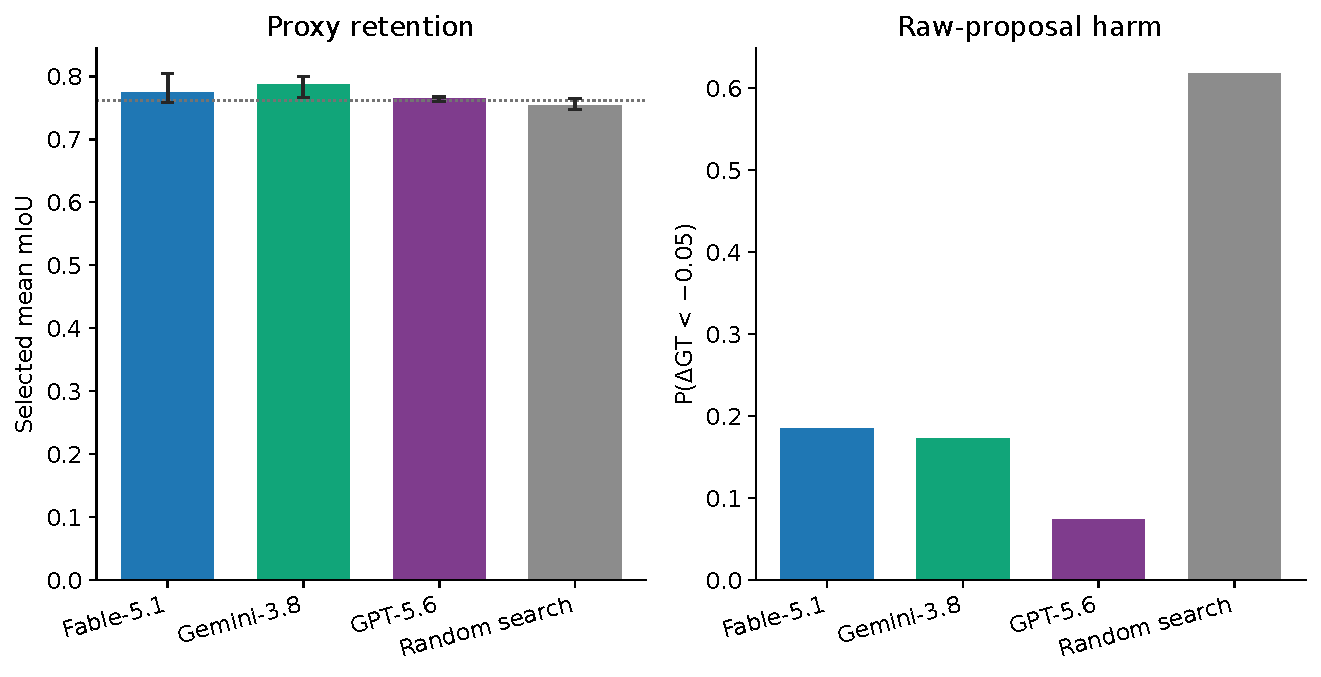
\includegraphics[width=0.98\linewidth]{figs/assume_random_comparison.pdf}
\end{hlbox}
\caption{\hl{Offline assumed-proxy selection for three LLM arms and adaptive-random search, with raw-proposal harm shown separately.}}\label{fig:assume-random-comparison}
\end{figure*}

\hl{From mean start mIoU} $\hl{0.762}$\hl{, assumed-proxy selection reaches} $\hl{0.765}$ \hl{for GPT-5.6,} $\hl{0.774}$ \hl{for Fable-5.1, and} $\hl{0.787}$ \hl{for Gemini-3.8. Adaptive-random selection instead reaches} $\hl{0.754}$ \hl{(Table}~\ref{tab:arm-compare}\hl{). All three LLM arms retain higher mean accuracy, although individual subsets deteriorate. Across all raw proposals,} $\hl{7}$\hl{--}$\hl{19\%}$ \hl{of LLM proposals are harmful, compared with} $\hl{62\%}$ \hl{for adaptive-random; this safety comparison is GT-based and proxy-independent.}

\hl{The same candidates show that proxy retention materially limits random-search damage, while selected losses in Table}~\ref{tab:arm-compare} \hl{show that increasing proxy score can still reduce true accuracy.}

\hl{Selected gains concentrate in the six starts below GT mIoU} $\hl{0.7}$\hl{, while the 21 stronger starts are flat or slightly negative (Table}~\ref{tab:gain-concentration}\hl{). This split is retrospective and does not control admission or selection.}

\begin{table*}[t]
\caption{\hl{Selected mIoU gain by initial-accuracy region; LOPO is the leave-one-parent-out range of mean gain.}}\label{tab:gain-concentration}
\begin{tabular*}{\textwidth}{@{\extracolsep{\fill}} l cccc @{}}
\toprule
Arm & Start $<0.7$ ($n=6$) & Start $\geq0.7$ ($n=21$) & Spearman(start, gain) & LOPO \\
\midrule
\rowcolor{yellow!25}Fable-5.1 & $+0.078$ & $-0.006$ & $-0.252$ & 0.004--0.026 \\
\rowcolor{yellow!25}Gemini-3.8 & $+0.143$ & $-0.009$ & $-0.406$ & 0.017--0.029 \\
\rowcolor{yellow!25}GPT-5.6 & $+0.010$ & $+0.001$ & $-0.258$ & 0.001--0.004 \\
\rowcolor{yellow!25}Random search & $+0.001$ & $-0.011$ & $-0.252$ & $-0.010$--$-0.005$ \\
\bottomrule
\end{tabular*}
\end{table*}

\begin{figure*}[t]
\centering
\begin{hlbox}
\centering
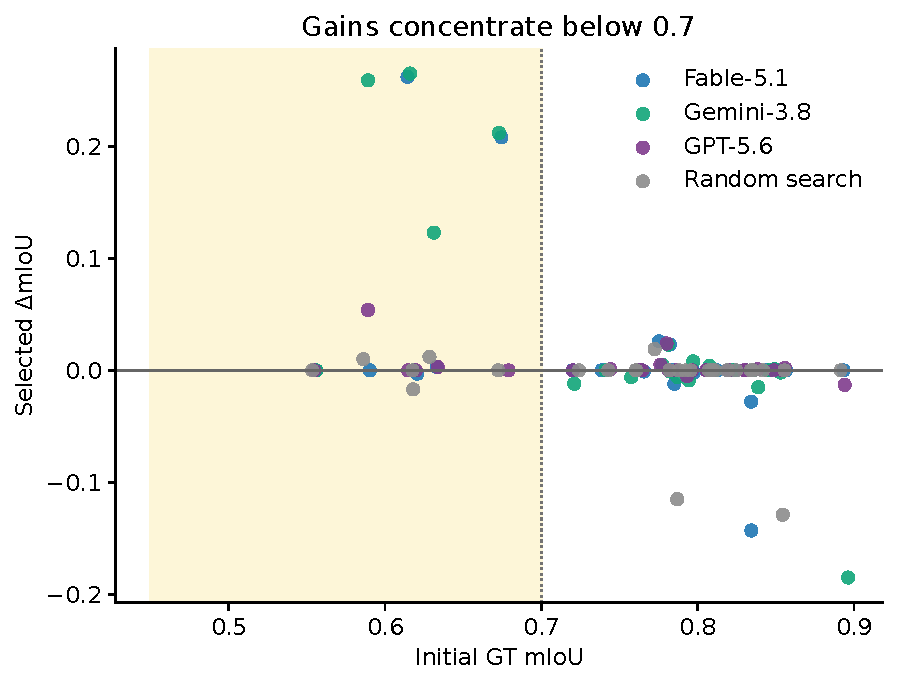
\includegraphics[width=0.98\linewidth]{figs/assume_gain_concentration.pdf}
\end{hlbox}
\caption{\hl{Selected mIoU gain versus initial mIoU; the shaded region marks the six starts below 0.7.}}\label{fig:assume-gain-concentration}
\end{figure*}


\subsection{Error analysis: block-identity shifts}
\label{sec:error-analysis}

\hl{In case 1-5, Fable-5.1 and Gemini-3.8 increase GT mIoU from} $\hl{0.676}$ \hl{to} $\hl{0.884}$ \hl{and} $\hl{0.888}$\hl{, while assumed-proxy score moves only from} $\hl{0.610}$ \hl{to} $\hl{0.636}$ \hl{and} $\hl{0.644}$\hl{. The accuracy gain is dominated by fewer swapped block identities rather than major changes in coverage.}

The K-block position anchors the assignment of block identities around each ring. Incorrect K-block localisation can therefore shift the label sequence while leaving the geometric boundaries largely unchanged. \hl{Such errors may preserve coverage, depth completeness, assumed-line count, and joint--boundary agreement, limiting the four-feature proxy's ability to distinguish correct boundaries from correct identities.} The largest losses for Fable-5.1 and Gemini-3.8 likewise show that a higher proxy score can accompany lower GT accuracy (Table~\ref{tab:arm-compare}). This limitation points to more reliable K-block localisation or independent evidence of block identity; a coherence metric derived from the same incorrect layout may remain insensitive to the error.

\subsection{Unseen-tunnel control}
\label{sec:stsd-control}

\hl{On one unseen STSD tunnel, nine controlled proposals were evaluated from a fixed intermediate state (proxy} $\hl{0.5578}$\hl{, zero assumed lines, first-10 mIoU} $\hl{0.7277}$\hl{). Eight were rejected and one was retained at proxy} $\hl{0.5664}$\hl{, zero assumed lines, and mIoU} $\hl{0.7276}$\hl{. This is initial retention evidence without an STSD-specific reference, not a second panel benchmark; the nine-row audit is in Appendix}~\ref{app:stsd-control}\hl{.}




% ══════════════════════════════════════════════════════════════════════════
\section{Discussion}\label{sec:discussion}
% ══════════════════════════════════════════════════════════════════════════

The results answer the research question of Section~\ref{sec:intro} in two parts. Intermediate metrics do carry accuracy information that survives transfer to \hl{held-out tunnel sections} and, less evenly, to unseen families. \hl{Proxy-based retention reduces losses relative to accepting proposals unconditionally, but selection errors can still reduce true accuracy. Final performance depends on both proposal quality and proxy accuracy.}

\subsection{Key findings}

\textbf{Fewer features transfer better.} \hl{After the post-hoc assumed-line substitution, the compact model reaches LOFO} $\rho=\hl{0.754}$\hl{, compared with} $\hl{0.744}$ \hl{for all ten revised features. With 120 runs from three development subsets, transfer rather than calibration fit remains the objective. The cost is coverage: the four retained features do not detect a block-identity shift.}

\textbf{Retention limits losses and can still select a worse output.} \hl{Offline assumed-proxy selection raises all three LLM means but reduces adaptive-random from} $\hl{0.762}$ \hl{to} $\hl{0.754}$\hl{. Selection errors still reduce true accuracy, so final performance depends on both proposal quality and proxy accuracy.} The same rule retains the losses in Table~\ref{tab:arm-compare}. The control compares proposal strategies under the same bounds, attempt budget, and selection rule; it does not isolate the use of pipeline evidence from differences in proposal size or parameter choice (Section~\ref{sec:agent-design}).

\textbf{What deployment would look like.} Each pipeline release still needs one expert reference per family and one calibration pass. From then on the frozen proxy supplies a label-free score that can be monitored over time and used as the selection signal inside a bounded self-refinement loop. \hl{Here, the} $\hl{0.4}$ \hl{threshold flags all constructed degradations and all 18 naturally occurring proposals below GT mIoU} $\hl{0.3}$\hl{, but the threshold was selected retrospectively and is not a certified deployment cutoff.} Self-refinement is assisted, auditable reconfiguration against a strong engineering baseline, not autonomous inspection.

\subsection{Comparison with state-of-the-art}\label{sec:positioning}
\begin{table*}[t]
\caption{Positioning Proxy4Tun against representative tunnel-segmentation paradigms. The comparison concerns setup cost and deployment capability as well as accuracy. mIoU figures are \emph{not} measured under comparable settings: supervised and expert-tuned figures are taken from prior work under their original protocols, whereas Proxy4Tun figures are from this study (27 held-out family-specific references).}\label{tab:sota}
\begin{tabular*}{\textwidth}{@{\extracolsep{\fill}} l c c c l @{}}
\toprule
Method & \begin{tabular}[t]{@{}c@{}}Deep learning\\training\end{tabular} & \begin{tabular}[t]{@{}c@{}}Per-case\\tuning\end{tabular} & \begin{tabular}[t]{@{}c@{}}Deployment-label-free\\quality signal\end{tabular} & mIoU (setting) \\
\midrule
LiningNet/SparseUNet/SCF-Net/FA-ResNet & \checkmark & -- & -- & 0.83--0.90 \\
SAM4Tun & -- & Expert & -- & above 0.90 \\
\rowcolor{yellow!25}\textbf{Proxy4Tun} (four-feature + LLM) & -- & \textbf{Auto} & \checkmark & \textbf{0.765--0.787} \\
\bottomrule
\end{tabular*}
\end{table*}

Comparisons here concern operating points, not accuracy leaderboards (Table~\ref{tab:sota}). Supervised 3D models on Seg2Tunnel report strong in-distribution accuracy~\cite{lin2024seg2tunnel} but require per-point labels and provide no deployment-time accept/refine/flag gate. Expert-tuned SAM4Tun reaches high accuracy on curated rings~\cite{ye2025sam4tun}, but a fixed configuration emits no signal when it degrades. Relative to that static pipeline, Proxy4Tun adds an explicit quality signal and a bounded self-refinement loop. The only directly comparable contrast in this study is LLM-plus-proxy versus random-plus-proxy under the shared reference starts and selection rule. The mIoU gap to expert-tuned SAM4Tun in Table~\ref{tab:sota} is therefore not a like-for-like deficit: those figures come from curated rings with per-case expert tuning, whereas the Proxy4Tun figures are 27 \hl{held-out subsets} with three automated attempts each.

\subsection{Limitations}\label{sec:limitations}

\hl{Five limitations bound the claims. First, 120 calibration runs come from three development subsets, and continuous-family LOFO remains weak} ($\rho=\hl{0.479}$)\hl{. Second, the assumed-line substitution and candidate reselection are post hoc; they rescore completed campaigns rather than rerun a closed loop with this proxy. Third, block-identity shifts remain weakly observed, so a higher proxy score can accompany lower GT accuracy. Fourth, the 324 natural proposals arise from bounded refinement rather than an independent deployment stream, and only five parent tunnels support the uncertainty estimates. Fifth, the STSD result is one control without an STSD-specific reference, not a general external benchmark.}


% ══════════════════════════════════════════════════════════════════════════
\section{Conclusions}\label{sec:conclusions}
% ══════════════════════════════════════════════════════════════════════════

This paper asked whether intermediate tunnel-segmentation metrics can estimate accuracy and guide parameter self-refinement on \hl{held-out tunnel sections} without new GT labels. \hl{The revision answers with an assumed-line four-feature Ridge proxy fitted only to the 120 calibration runs and applied offline to saved held-out and refinement artifacts.}

\begin{itemize}
\item \hl{The assumed-line proxy reaches Spearman} $\hl{0.789}$ \hl{on 54 held-out runs and orders every reference above its degraded partner; compact LOFO is} $\hl{0.754}$\hl{.}
\item \hl{From a} $\hl{0.762}$ \hl{baseline, offline assumed-proxy selection reaches} $\hl{0.765}$\hl{--}$\hl{0.787}$ \hl{for the three LLM arms, while adaptive-random reaches} $\hl{0.754}$\hl{. Gains concentrate on six starts below mIoU} $\hl{0.7}$\hl{.}
\item \hl{Final performance depends on both proposal quality and proxy accuracy.}
\end{itemize}

\hl{The principal remaining limit is a block-identity shift: the four features can approve an output whose K-block localisation is wrong. Future work should add independent block-identity evidence, test the assumed-line proxy prospectively on naturally degraded deployment streams and more external tunnels, and examine refinement without an expert reference.} Until then, Proxy4Tun is a label-free assessment and assisted-reconfiguration tool, not an autonomous inspector.

% ══════════════════════════════════════════════════════════════════════════
% Data availability, declarations, etc.
% ══════════════════════════════════════════════════════════════════════════

\section*{Data availability}

\hl{The source code, parameter snapshots, frozen saved runs, assumed-line rescoring script, provenance table, and evaluation outputs will be released upon publication.} The Seg2Tunnel dataset is publicly available~\cite{lin2024seg2tunnel}.

\section*{Declaration of competing interest}

The authors declare that they have no known competing financial interests or personal relationships that could have appeared to influence the work reported in this paper.

\section*{Declaration of generative AI use}

During this study, LLM agents (GPT-5.6, Fable-5.1, and Gemini-3.8) were evaluated as proposal mechanisms in the self-refinement loop, together with a random-search control under the same proxy-based selection rule. LLMs were also used for language editing and for improving manuscript structure. The authors reviewed and edited all content and take full responsibility for the content of the publication.

% ══════════════════════════════════════════════════════════════════════════
% Bibliography
% ══════════════════════════════════════════════════════════════════════════

% Natbib requires a BibTeX style; without it, citations stay as “?”
% NOTE: \balance can cause column-balancing artefacts in the reference list (e.g.,
% lines slipping into the footer area) with this class. Keep it off for the bibliography.
%\balance
\bibliographystyle{model1-num-names}
\bibliography{references}


% ══════════════════════════════════════════════════════════════════════════
% Appendix
% ══════════════════════════════════════════════════════════════════════════

\appendix

\section{Pipeline anchor parameters}\label{app:anchor-parameter}

This appendix summarises the expert-tuned \emph{anchor} parameter profiles used to warm-start the segmentation pipeline for each lining family (staggered, continuous, complex). Table~\ref{tab:anchor-params} lists the fixed stage algorithms and the corresponding family-specific parameter values that define the reference configurations used throughout the study.

\begin{table*}[t]
\caption{Pipeline anchor parameters: expert-tuned, family-specific anchor parameter profiles of the segmentation pipeline.}\label{tab:anchor-params}
\begin{tabular*}{\textwidth}{@{\extracolsep{\fill}} l l p{0.30\textwidth} l @{}}
\toprule
Stage & Parameter & Description & Staggered / Continuous / Complex \\
\midrule
Unfolding & \texttt{diameter} & Cylindrical scale. & 5.5 / 5.9 / 7.5\,m \\
Unfolding & \texttt{slice\_spacing\_factor} & Slice spacing (ring width). & 1.2 / 1.2 / 1.8\,m \\
Unfolding & \texttt{polynomial\_degree} & Centreline fit degree. & 3 / 2 / 2 \\
Unfolding & \texttt{residual\_recentre} & Per-bin frame recentring. & off / on / on \\
\midrule
Denoising & \texttt{mask\_r\_low} & Inner radial gate. & 2.33 / 2.85 / 3.65\,m \\
Denoising & \texttt{mask\_r\_high} & Outer radial gate. & 2.78 / 3.0 / 3.9\,m \\
Denoising & \texttt{y\_step} & Angular bin width. & 0.4 / 0.5 / 0.1\,m \\
Denoising & \texttt{z\_step} & Radial histogram bin width. & 0.005 / 0.001 / 0.001\,m \\
Denoising & \texttt{grad\_threshold} & Outer-edge gradient threshold. & 0.15 / 0.2 / 0.2 \\
Denoising & \texttt{smoothing\_window\_size} & Cutoff-curve smoothing window. & 5 / 3 / 3 \\
Denoising & \texttt{smoothing\_offset} & Post-smoothing cutoff bias. & $-$0.002 / $-$0.003 / $-$0.005\,m \\
Denoising & \texttt{default\_cutoff\_z} & Fallback radial cutoff. & 2.75 / 2.85 / 3.65\,m \\
\midrule
Enhancing & \texttt{upsampling\_stage1} & Stage-1 upsampling spacing. & 0.06 / 0.08 / 0.09\,m \\
Enhancing & \texttt{upsampling\_stage2} & Stage-2 upsampling spacing. & 0.03 / 0.04 / 0.045\,m \\
Enhancing & \texttt{upsampling\_stage3} & Stage-3 upsampling spacing. & 0.015 / 0.02 / 0.0225\,m \\
Enhancing & \texttt{curvature\_threshold} & Panel--joint curvature threshold. & 0.005 / 0.0005 / 0.0005 \\
Enhancing & \texttt{depth\_threshold\_low} & Lower interpolation depth tolerance. & 0.005 / 0.01 / 0.0065\,m \\
Enhancing & \texttt{depth\_threshold\_high} & Upper interpolation depth tolerance. & 0.015 / 0.01 / 0.013\,m \\
Enhancing & \texttt{inter\_radius} & Interpolation neighbour radius. & 0.03 / 0.06 / 0.06\,m \\
Enhancing & \texttt{n\_segment\_start/end} & Interpolated ring-index window. & 0--5 / 2--8 / 5--14 \\
Enhancing & \texttt{ring\_spacing\_factor} & Nominal ring width. & 1.2 / 1.2 / 1.8\,m \\
\midrule
Detecting & \texttt{binary\_threshold} & Depth-map binarisation level. & 125 / 127 / 125 \\
Detecting & \texttt{hough\_thresh\_obliq} & Oblique joint-line vote threshold. & 65 / 30 / 35 \\
Detecting & \texttt{hough\_thresh\_horiz} & Horizontal joint-line vote threshold. & 65 / 30 / 35 \\
Detecting & \texttt{hough\_thresh\_vert} & Ring-boundary vote threshold. & 600 / 1500 / 5000 \\
Detecting & \texttt{minLineLength\_obliq} & Minimum oblique line length. & 100 / 40 /  80\,px \\
Detecting & \texttt{minLineLength\_horiz} & Minimum horizontal line length. & 100 / 50 /  80\,px \\
Detecting & \texttt{maxLineGap\_obliq} & Oblique line-merging gap limit. & 45 / 30 /  60\,px \\
Detecting & \texttt{maxLineGap\_horiz} & Horizontal line-merging gap limit. & 10 / 10 /  15\,px \\
Detecting & \texttt{angle\_range\_oblique} & Oblique-joint angle band. & $\pm$[6, 9] / $\pm$[4, 10] / $\pm$[5, 10]$^{\circ}$ \\
\midrule
Segmenting & \texttt{segment\_per\_ring} & Segments per lining ring. & 6 / 6 / 7 \\
Segmenting & \texttt{segment\_order} & Circumferential segment order. & \begin{tabular}[t]{@{}l@{}}K,B1,A1--A3,B2 /\\K,B2,A3--A1,B1 /\\K,B1,A1--A4,B2\end{tabular} \\
Segmenting & \texttt{segment\_width} & Nominal segment width. & 1200 / 1200 / 1800\,mm \\
Segmenting & \texttt{K\_height} & Key-segment arc height. & 1079.9 / 823.8 / 1227.0\,mm \\
Segmenting & \texttt{AB\_height} & Standard-segment arc height. & 3239.8 / 3346.8 / 3726.9\,mm \\
Segmenting & \texttt{angle} & Oblique K-joint inclination. & 7.52 / 6.12 / 9.8$^{\circ}$ \\
Segmenting & \texttt{processing.y\_bounds} & Valid panorama band. & 3800--13300 / 4500--14000 / 4200--13100\,px \\
\bottomrule
\end{tabular*}
\end{table*}

\section{Bayesian exploration configuration}\label{app:bo-config}

Table~\ref{tab:bo-config} records the frozen design-time exploration settings
used to generate the 120 calibration trials. Accepted trials are exactly
$N_0{=}32$ Sobol $+\,N_{\mathrm{GP}}{=}8$ GP-uncertainty acquisitions per family
(40 valid trials each).

\begin{table*}[t]
\caption{Design-time Bayesian exploration configuration (frozen snapshot).}\label{tab:bo-config}
\begin{tabular*}{\textwidth}{@{\extracolsep{\fill}} l l @{}}
\toprule
Setting & Value \\
\midrule
Target accepted trials / family & $N{=}40$ ($N_0{=}32$ Sobol, $N_{\mathrm{GP}}{=}8$ accepted GP) \\
Sobol & Scrambled QMC in the unit cube \\
GP kernel & Mat\'{e}rn $\nu{=}2.5$ $+$ white noise; \texttt{normalize\_y=True} \\
Length-scale bounds & $(10^{-2},10^{2})$ per dimension; noise $(10^{-6},10^{-1})$ \\
GP optimiser & \texttt{GaussianProcessRegressor}, $n_{\mathrm{restarts\_optimizer}}{=}3$ \\
Acquisition & Maximise predictive std over random candidate pool $\mathcal{P}_{\mathrm{BO}}$ of size $2048$ \\
Failure / top-up rule & Status not ok or required features incomplete $\Rightarrow$ exclude; continue until accepted targets met \\
\bottomrule
\end{tabular*}
\end{table*}

\section{Per-family search-space bounds}\label{app:search-bounds}

This appendix reports the full bounded per-family search spaces $B$ used for Bayesian exploration. Table~\ref{tab:bo-bounds} enumerates every optimised parameter and its allowable range (or discrete set) for each family reference case, defining the constraints enforced during the frozen 120-trial campaign.

\begin{table*}[t]
\caption{Complete per-family search-space bounds $B$ for the frozen 120-trial campaign.}\label{tab:bo-bounds}
{\small
\begin{tabular*}{\textwidth}{@{\extracolsep{\fill}} llp{0.28\textwidth} @{}}
\toprule
Family (case) & Parameter & Bounds \\
\midrule
Staggered (2-1) & \texttt{unfolding.ransac\_threshold} & $[0.8,1.2]$ \\
 & \texttt{unfolding.slice\_spacing\_factor} & $[1.05,1.35]$ \\
 & \texttt{unfolding.polynomial\_degree} & $\{2,3\}$ \\
 & \texttt{unfolding.random\_seed} & $\{0,\ldots,7\}$ \\
 & \texttt{denoising.mask\_r\_low} & $[2.2,2.5]$ \\
 & \texttt{denoising.mask\_r\_high} & $[2.7,2.9]$ \\
 & \texttt{denoising.z\_step} & $[0.001,0.008]$ \\
 & \texttt{denoising.grad\_threshold} & $[0.1,0.25]$ \\
 & \texttt{enhancing.curvature\_threshold} & $[3{\times}10^{-4},8{\times}10^{-3}]$ \\
 & \texttt{enhancing.inter\_radius} & $[0.02,0.08]$ \\
 & \texttt{detecting.binary\_threshold} & $[100,160]$ \\
 & \texttt{detecting.hough\_threshold\_oblique} & $[40,90]$ \\
 & \texttt{detecting.hough\_threshold\_horizontal} & $[40,90]$ \\
 & \texttt{detecting.hough\_threshold\_vertical} & $[400,800]$ \\
 & \texttt{detecting.maxLineGap\_oblique} & $[20,80]$ \\
 & \texttt{sam.y\_bounds\_lower} & $[3600,4400]$ \\
\addlinespace
Continuous (3-1) & \texttt{unfolding.ransac\_threshold} & $[0.8,1.2]$ \\
 & \texttt{unfolding.slice\_spacing\_factor} & $[1.05,1.35]$ \\
 & \texttt{unfolding.polynomial\_degree} & $\{2,3\}$ \\
 & \texttt{unfolding.random\_seed} & $\{0,\ldots,7\}$ \\
 & \texttt{denoising.mask\_r\_low} & $[2.7,3.0]$ \\
 & \texttt{denoising.mask\_r\_high} & $[2.9,3.15]$ \\
 & \texttt{denoising.mask\_theta\_low} & $[1.0,2.5]$ \\
 & \texttt{denoising.mask\_theta\_high} & $[15,19]$ \\
 & \texttt{enhancing.curvature\_threshold} & $[2{\times}10^{-4},2{\times}10^{-3}]$ \\
 & \texttt{detecting.binary\_threshold} & $[100,160]$ \\
 & \texttt{detecting.hough\_threshold\_oblique} & $[20,60]$ \\
 & \texttt{detecting.hough\_threshold\_horizontal} & $[20,60]$ \\
 & \texttt{detecting.hough\_threshold\_vertical} & $[800,2500]$ \\
 & \texttt{detecting.maxLineGap\_oblique} & $[10,60]$ \\
 & \texttt{detecting.pattern\_tolerance} & $[5,20]$ \\
 & \texttt{detecting.uniform\_k\_snap} & $\{\mathrm{off},\mathrm{on}\}$ \\
 & \texttt{sam.segment\_width} & $[1000,1400]$ \\
 & \texttt{sam.K\_height} & $[700,1000]$ \\
 & \texttt{sam.angle} & $[4,9]$ \\
\addlinespace
Complex (5-1) & \texttt{unfolding.ransac\_threshold} & $[0.8,1.2]$ \\
 & \texttt{unfolding.slice\_spacing\_factor} & $[1.6,2.0]$ \\
 & \texttt{unfolding.polynomial\_degree} & $\{2,3\}$ \\
 & \texttt{unfolding.random\_seed} & $\{0,\ldots,7\}$ \\
 & \texttt{denoising.mask\_r\_low} & $[3.5,3.8]$ \\
 & \texttt{denoising.mask\_r\_high} & $[3.75,4.05]$ \\
 & \texttt{enhancing.curvature\_threshold} & $[2{\times}10^{-4},2{\times}10^{-3}]$ \\
 & \texttt{detecting.binary\_threshold} & $[100,160]$ \\
 & \texttt{detecting.hough\_threshold\_oblique} & $[25,70]$ \\
 & \texttt{detecting.hough\_threshold\_horizontal} & $[25,70]$ \\
 & \texttt{detecting.hough\_threshold\_vertical} & $[800,5000]$ \\
 & \texttt{detecting.maxLineGap\_oblique} & $[30,80]$ \\
 & \texttt{detecting.maxLineGap\_horizontal} & $[5,30]$ \\
 & \texttt{detecting.pattern\_tolerance} & $[5,20]$ \\
 & \texttt{sam.segment\_width} & $[1500,2100]$ \\
 & \texttt{sam.K\_height} & $[1000,1500]$ \\
 & \texttt{sam.angle} & $[7,12]$ \\
\bottomrule
\end{tabular*}}
\end{table*}


\section{Tunnel ontology structure}\label{app:ontology}

The reflective agent consults a staged SAM4Tun ontology that encodes pipeline
artifacts, per-stage parameters and quality metrics, failure modes, diagnostic
rules, remediation actions, and inter-stage dependencies. The top-level schema
is summarised below:
We omit the complete YAML and show only the structure plus one representative
stage example.

\begin{lstlisting}[caption={Ontology top-level keys and stage inventory.},label={lst:ontology-structure}]
meta                  # version, domain, coordinate systems
artifacts             # data objects (cloud, depth map, masks, ...)
stages[]              # pipeline stages (unfolding through segmentation):
  stage_1_centreline
  stage_2_denoise
  stage_3_upsample
  stage_4_detection
  stage_5_segmentation
inter_stage_dependencies[]   # upstream cause -> defer local retune
diagnostic_rules[]           # metric patterns -> failure modes
remediation_actions[]        # bounded parameter changes
agent_interface              # {state, diagnosis, proposal}
\end{lstlisting}

\begin{lstlisting}[caption={Example ontology stage: radial denoising failure modes.},label={lst:ontology-example}]
- id: stage_2_denoise
  name: Local density-difference-based denoising
  quality_metrics:
    - id: m_retained_ratio
      healthy: "lining kept; background removed"
    - id: m_bg_leakage
      healthy: "near zero"
  failure_modes:
    - id: f_over_gate
      name: Radial gate too tight
      symptom: "lining removed; holes in later depth map"
    - id: f_under_gate
      name: Radial gate too loose
      symptom: "rails/tube/noise retained downstream"
\end{lstlisting}

\section{Agent prompt structure}\label{app:prompt}

Each reflection round issues a single bounded JSON overlay. The model-facing
prompt is assembled from a fixed skeleton (role, isolation rules, current
state, GT-blind intrinsics, four-feature proxy scores, allowed artifact images,
family parameter bounds, and the required output schema). Listing~\ref{lst:prompt-skeleton}
summarises the skeleton; Listing~\ref{lst:prompt-example} gives one example
proposal. GT mIoU and evaluation directories are never included.

\begin{lstlisting}[caption={Agent-prompt skeleton (per round).},label=lst:prompt-skeleton]
Role: reflective parameter agent for SAM4Tun
Allowed context:
  - family reference priors / warm-start parameters
  - GT-blind intrinsics and four-feature proxy scores
  - stage artifacts (depth map, detections, SAM masks)
  - ontology + bounded family search space
State: subset, family, reference proxy, operating band
Task: diagnose failure mode; propose ONE overlay within bounds
Output JSON keys (required):
  observation, failure_mode, rationale, overlay
\end{lstlisting}

\begin{lstlisting}[caption={Example JSON proposal returned by the agent.},label=lst:prompt-example]
{
  "observation": "Centreline residual is high; unroll shows asymmetric voids.",
  "failure_mode": "f_curve_underfit (under-fit centre curve)",
  "rationale": "Raise polynomial degree and tighten RANSAC before retuning SAM.",
  "overlay": {
    "unfolding": {
      "polynomial_degree": 3,
      "ransac_threshold": 0.9
    }
  }
}
\end{lstlisting}

\section{Random-search control}\label{app:random-search}

The random-search control samples sparse overlays. Let $k$ be the number of parameters changed in a round. We draw $k$ from a frozen empirical distribution estimated from an earlier LLM pilot campaign (198 proposals across three LLM arms), then sample $k$ distinct parameters uniformly (without replacement) from the bounded search space and sample each chosen parameter value uniformly within its family-specific bounds. That pilot distribution does not match the present LLM proposals: this experiment records a mean of $8.64$ changed parameters for random against $4.11$--$7.35$ for the LLM arms. Unfolding parameters are eligible only when the start's centreline residual exceeds 10\,cm, matching the constraint applied to LLM arms. Parameter identities and values are otherwise random; the overlay is applied to the retained configuration, and retention uses the proxy score. The distribution and seed were frozen before any LLM attempt in this study, so the control cannot track the LLM runs it is compared with.

\begin{hlbox}
\noindent\textbf{Frozen sampling design.} Seed base $20260915$; the generator for case index $i$ and round $r$ is seeded with $20260915+1000\,i+r$. Change-count probabilities $\Pr(k)$, $k=1,\ldots,15$:
\begin{center}
\small
\setlength{\tabcolsep}{3.5pt}
\begin{tabular}{@{}l cccccccc@{}}
\toprule
$k$ & 1 & 2 & 3 & 4 & 5 & 6 & 7 & 8 \\
$\Pr(k)$ & .036 & .005 & .025 & .030 & .046 & .061 & .066 & .051 \\
\midrule
$k$ & 9 & 10 & 11 & 12 & 13 & 14 & 15 & \\
$\Pr(k)$ & .076 & .071 & .157 & .188 & .107 & .076 & .005 & \\
\bottomrule
\end{tabular}
\end{center}
A draw of $k$ larger than the number of eligible parameters is clipped to that number.
\end{hlbox}

\section{Predefined parameter perturbations}\label{app:degradation}

Each held-out subset is paired with one family-specific overlay taken from the lowest-GT-mIoU valid calibration trial of that family's development subset. Unfolding keys are dropped so the perturbation does not change the centreline; the remaining stage-2 to stage-5 keys are applied to the family reference. The three overlays were frozen before any held-out scoring. All 54 runs completed, so no perturbation was replaced.

\begin{hlbox}
\small
\noindent\textbf{Staggered} (source 2-1/s017, source GT mIoU $0.032$).
\texttt{mask\_r\_low}$=2.207$,
\texttt{mask\_r\_high}$=2.741$,
\texttt{z\_step}$=0.00633$,
\texttt{grad\_threshold}$=0.183$,
\texttt{curvature\_threshold}$=7.14\times10^{-4}$,
\texttt{inter\_radius}$=0.0353$,
\texttt{binary\_threshold}$=125$,
\texttt{hough\_threshold\_oblique}$=46$,
\texttt{hough\_threshold\_horizontal}$=60$,
\texttt{hough\_threshold\_vertical}$=520$,
\texttt{maxLineGap\_oblique}$=36$,
\texttt{processing.y\_bounds}$=[4003,13100]$.

\medskip
\noindent\textbf{Continuous} (source 3-1/s030, source GT mIoU $0.042$).
\texttt{mask\_r\_low}$=2.756$,
\texttt{mask\_r\_high}$=2.906$,
\texttt{mask\_theta\_low}$=2.063$,
\texttt{mask\_theta\_high}$=18.79$,
\texttt{curvature\_threshold}$=1.55\times10^{-3}$,
\texttt{binary\_threshold}$=106$,
\texttt{hough\_threshold\_oblique}$=32$,
\texttt{hough\_threshold\_horizontal}$=37$,
\texttt{hough\_threshold\_vertical}$=2457$,
\texttt{pattern\_tolerance}$=13$,
\texttt{segment\_width}$=1315$,
\texttt{K\_height}$=944$,
\texttt{angle}$=5.56^{\circ}$.

\medskip
\noindent\textbf{Complex} (source 5-1/g001, source GT mIoU $0.036$).
\texttt{mask\_r\_low}$=3.776$,
\texttt{mask\_r\_high}$=3.961$,
\texttt{curvature\_threshold}$=2.42\times10^{-4}$,
\texttt{binary\_threshold}$=159$,
\texttt{hough\_threshold\_oblique}$=33$,
\texttt{hough\_threshold\_horizontal}$=26$,
\texttt{hough\_threshold\_vertical}$=4596$,
\texttt{maxLineGap\_oblique}$=40$,
\texttt{maxLineGap\_horizontal}$=22$,
\texttt{pattern\_tolerance}$=15$,
\texttt{segment\_width}$=1847$,
\texttt{K\_height}$=1014$,
\texttt{angle}$=8.35^{\circ}$.
\end{hlbox}

\section{\hl{Assumed-line proxy scaling}}\label{app:assumed-proxy}

\begin{table}[ht]
\caption{\hl{Frozen standardisation and coefficients fitted on the 120 calibration records. The intercept is 0.358867 and Ridge} $\alpha=\hl{5.623413}$\hl{.}}\label{tab:assumed-proxy-scaling}
\begin{tabular*}{\tblwidth}{@{\extracolsep{\fill}} l ccc @{}}
\toprule
Feature & Mean & SD & Coefficient \\
\midrule
\rowcolor{yellow!25}Correspondence F1@15 & 0.1653 & 0.1517 & $+0.0884$ \\
\rowcolor{yellow!25}Fill rate & 0.4569 & 0.2836 & $+0.1058$ \\
\rowcolor{yellow!25}Assumed-line count & 4.5917 & 3.6595 & $-0.0216$ \\
\rowcolor{yellow!25}Missing-depth rate & 0.4075 & 0.3033 & $-0.0340$ \\
\bottomrule
\end{tabular*}
\end{table}

\section{\hl{Unseen-tunnel control audit}}\label{app:stsd-control}

\hl{The fixed starting context is proxy 0.5578, zero assumed lines, and first-10 mIoU 0.7277. It was selected after a longer-than-three-attempt exploration. The table reports only the nine controlled follow-up rows, not the complete trajectory or a global three-attempt budget.}

\begin{table*}[t]
\caption{\hl{STSD control from the fixed intermediate state.}}\label{tab:stsd-control}
{\footnotesize
\begin{tabular*}{\textwidth}{@{\extracolsep{\fill}} l c p{0.39\textwidth} l c c c @{}}
\toprule
Arm & Round & Overlay & Verdict & Proxy & Assumes & mIoU10 \\
\midrule
\rowcolor{yellow!25}GPT & 1 & \texttt{\{"detecting":\{"prompt\_logic":"notebook\_12"\}\}} & rejected & 0.5578 & 0 & 0.7277 \\
\rowcolor{yellow!25}GPT & 2 & \texttt{\{"sam":\{"AB\_height":3220.0\}\}} & rejected & 0.3601 & 0 & 0.7147 \\
\rowcolor{yellow!25}GPT & 3 & \texttt{\{"sam":\{"processing.y\_bounds":[3000,12900]\}\}} & rejected & 0.5326 & 0 & 0.7285 \\
\rowcolor{yellow!25}Gemini & 1 & \texttt{\{"detecting":\{"prompt\_logic":"t12\_pattern"\}\}} & rejected & 0.5218 & 0 & 0.6018 \\
\rowcolor{yellow!25}Gemini & 2 & \texttt{\{"sam":\{"processing.y\_bounds":[2800,13100]\}\}} & rejected & 0.5311 & 0 & 0.7292 \\
\rowcolor{yellow!25}Gemini & 3 & \texttt{\{"detecting":\{"key\_pair\_max\_sep\_px":300\}\}} & rejected & 0.5578 & 0 & 0.7277 \\
\rowcolor{yellow!25}Claude & 1 & \texttt{\{"sam":\{"processing.padding":250\}\}} & rejected & 0.5280 & 0 & 0.7293 \\
\rowcolor{yellow!25}Claude & 2 & \texttt{\{"sam":\{"processing.y\_bounds":[2800,13100]\}\}} & rejected & 0.5311 & 0 & 0.7292 \\
\rowcolor{yellow!25}Claude & 3 & \texttt{\{"sam":\{"angle":8.0\}\}} & accepted & 0.5664 & 0 & 0.7276 \\
\bottomrule
\end{tabular*}}
\end{table*}

\begin{figure*}[t]
\centering
\begin{hlbox}
\centering
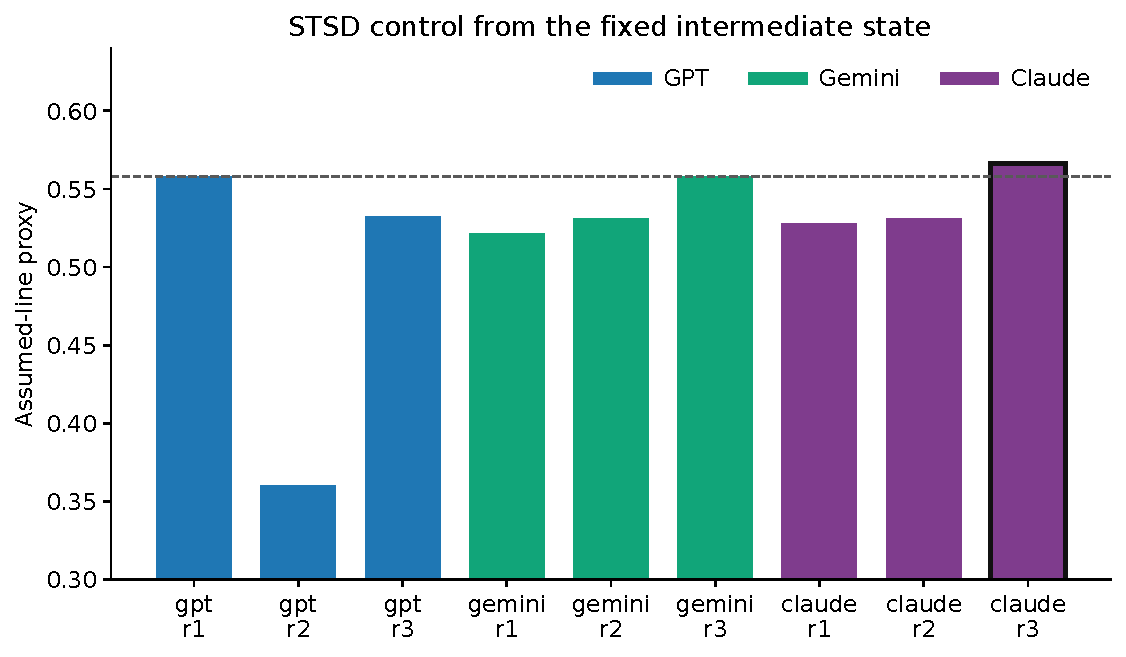
\includegraphics[width=0.98\linewidth]{figs/assume_stsd_control.pdf}
\end{hlbox}
\caption{\hl{Assumed-line proxy, first-10 mIoU, and assumed-line outcomes for the nine-row STSD control.}}\label{fig:assume-stsd-control}
\end{figure*}

\section{Full-panel selection audit}\label{app:poc-selection}

\hl{Table}~\ref{tab:panel-audit} \hl{summarises assumed-proxy offline selection for all 27 held-out references. Among candidates within} $\hl{0.01}$ \hl{of the maximum score, the earliest round is selected.}

\begin{table*}[t]
\caption{\hl{Merged 27-case panel after assumed-line proxy reselection: reference start and selected GT mIoU by arm.}}\label{tab:panel-audit}
{\footnotesize
\begin{tabular*}{\textwidth}{@{\extracolsep{\fill}} l l c cccc @{}}
\toprule
Subset & Family & Start & GPT-5.6 & Fable-5.1 & Gemini-3.8 & Random \\
\midrule
1-1 & staggered & 0.784 & 0.784 & 0.784 & 0.783 & 0.784 \\
1-2 & staggered & 0.809 & 0.809 & 0.809 & 0.809 & 0.809 \\
1-3 & staggered & 0.827 & 0.827 & 0.827 & 0.827 & 0.827 \\
\rowcolor{yellow!25}1-4 & staggered & 0.853 & 0.855 & 0.853 & 0.851 & 0.853 \\
1-5 & staggered & 0.676 & 0.676 & 0.884 & 0.888 & 0.676 \\
2-2 & staggered & 0.615 & 0.615 & 0.877 & 0.880 & 0.615 \\
\rowcolor{yellow!25}2-3 & staggered & 0.795 & 0.790 & 0.793 & 0.803 & 0.795 \\
2-4 & staggered & 0.835 & 0.835 & 0.807 & 0.835 & 0.835 \\
2-5 & staggered & 0.893 & 0.880 & 0.893 & 0.708 & 0.893 \\
3-2 & continuous & 0.631 & 0.634 & 0.634 & 0.754 & 0.643 \\
\rowcolor{yellow!25}3-3 & continuous & 0.808 & 0.808 & 0.808 & 0.812 & 0.808 \\
3-4 & continuous & 0.622 & 0.622 & 0.619 & 0.622 & 0.605 \\
3-5 & continuous & 0.588 & 0.642 & 0.588 & 0.847 & 0.598 \\
3-6 & continuous & 0.836 & 0.837 & 0.693 & 0.821 & 0.836 \\
\rowcolor{yellow!25}3-7 & continuous & 0.845 & 0.845 & 0.845 & 0.845 & 0.845 \\
\rowcolor{yellow!25}3-8 & continuous & 0.723 & 0.723 & 0.723 & 0.711 & 0.723 \\
3-9 & continuous & 0.820 & 0.820 & 0.820 & 0.820 & 0.820 \\
\rowcolor{yellow!25}3-10 & continuous & 0.853 & 0.853 & 0.854 & 0.854 & 0.724 \\
\rowcolor{yellow!25}4-1 & complex & 0.741 & 0.742 & 0.741 & 0.741 & 0.741 \\
4-2 & complex & 0.787 & 0.787 & 0.775 & 0.781 & 0.787 \\
4-3 & complex & 0.554 & 0.554 & 0.554 & 0.554 & 0.554 \\
4-4 & complex & 0.784 & 0.808 & 0.807 & 0.807 & 0.669 \\
4-5 & complex & 0.808 & 0.808 & 0.808 & 0.808 & 0.808 \\
5-2 & complex & 0.793 & 0.793 & 0.793 & 0.784 & 0.793 \\
5-3 & complex & 0.762 & 0.762 & 0.761 & 0.762 & 0.762 \\
5-4 & complex & 0.760 & 0.760 & 0.760 & 0.754 & 0.760 \\
5-5 & complex & 0.775 & 0.780 & 0.801 & 0.780 & 0.794 \\
\midrule
\rowcolor{yellow!25}Mean & -- & 0.762 & 0.765 & 0.774 & 0.787 & 0.754 \\
\bottomrule
\end{tabular*}}
\end{table*}

\end{document}